\documentclass{sig-alternate}
\usepackage{epsfig}

%%  \toappear{
%%  %\raisebox{2pt}[2pt]{\underline{~~~~~~~~~~~~~~~~~~~~~~~~~~~~~~~~~~~~~~~~~~~~~~~~~~}} \\
%%  %$^*$ More information on the StreamIt project is available from
%%  %\texttt{http://compiler.lcs.mit.edu/streamit} \\
%%    \rule{0cm}{0cm}\\\hrule\rule{0cm}{0cm} ~ \\ \vspace{-6pt} ~ \\
%%  \parbox[b]{20pc}{\baselineskip 9pt
%%  Permission to make digital or hard copies of all or part of this work
%%  for personal or classroom use is granted without fee provided that
%%  copies are not made or distributed for profit or commercial advantage
%%  and that copies bear this notice and the full citation on the first
%%  page.  To copy otherwise, to republish, to post on servers or to
%%  redistribute to lists, requires prior specific permission and/or a
%%  fee.} \par
%%  {\it PLDI'03}, June 9--11, 2003, San Diego, California, USA. \par
%%  Copyright 2003 ACM 1-58113-662-5/03/0006 ...\$5.00 \\ ~ \\ ~ \\
%% }

%%  \conferenceinfo{PLDI'03}{June 9---11, 2003, San Diego, California, USA.}
%%  \CopyrightYear{2003}
%%  \crdata{1-58113-662-5/03/0006}

\title{Stream Dependence Analysis and its \\ Application to Precise Event Handling}
\numberofauthors{1}
\author{
	William Thies, Michal Karczmarek, Janis Sermulins, Rodric Rabbah, and Saman Amarasinghe\\
	\small MIT Computer Science and Artificial Intelligence Laboratory\\
	\small \{thies, karczma, janiss, rabbah, saman\}@csail.mit.edu
}


\begin{document}
\newtheorem{definition}{Definition}
\newtheorem{theorem}{Theorem}
\newtheorem{algorithm}{Algorithm}

\maketitle

\newcommand{\figsdep}[0]{\mt{SDEP}}
\newcommand{\figsdepf}[2]{\mt{SDEP}_{#1 \small{\leftarrow} #2}}
\newcommand{\sdep}[0]{\textsc{sdep}}
\newcommand{\sdepf}[2]{\sdep_{#1 \small{\leftarrow} #2}}
\newcommand{\floor}[2]{\left\lfloor\frac{#1}{#2}\right\rfloor}
\newcommand{\ceil}[2]{\left\lceil\frac{#1}{#2}\right\rceil}

\newcommand{\mt}[1]{\mbox{\it #1}}
\newcommand{\todo}[1]{\framebox{\bf #1}}
\newcommand{\naive}[0]{na\"{\i}ve}
\newcommand{\Naive}[0]{Na\"{\i}ve}
\newcommand{\makeline}[0]{\rule{0cm}{0cm}\\\hrule\rule{0cm}{0cm}}

\begin{abstract}
Due to the high data rates involved in audio, video, and signal
processing applications, it is imperative to compress the data to
decrease the amount of storage used.  Unfortunately, this implies that
any program operating on the data needs to be wrapped by a
decompression and re-compression stage.  Re-compression can incur
significant computational overhead, while decompression swamps the
application with the original volume of data.

In this paper, we present a program transformation that greatly
accelerates the processing of compressible data.  Given a program that
operates on uncompressed data, we output an equivalent program that
operates directly on the compressed format.  Our transformation
applies to stream programs, a restricted but useful class of
applications with regular communication and computation patterns.  Our
formulation is based on LZ77, a lossless compression algorithm
utilized by ZIP, and immediately applies to simpler formats such as
Apple Animation, Microsoft RLE, and Targa.

We implemented a simple subset of our techniques in the StreamIt
compiler, which emits executable plugins for two popular video editing
tools: MEncoder and Blender.  For common operations such as color
adjustment and video compositing, computing directly on compressed
data offers a speedup roughly proportional to the overall compression
ratio.  For our benchmark suite of 12 videos in Apple Animation
format, speedups range from 1.1x to 471x, with a median of 15x.

\end{abstract}

\section{Introduction}


Stream computing represents an increasingly important class of
applications. In streaming codes, there is an abundance of parallelism that
is easier to extract compared to traditional desktop workloads (e.g.,
pointer-based computing). As a result, the extraction of parallelism
in streaming codes does not require heroic efforts, and thus,
processors can deliver higher performance with significantly lower
power costs. This is especially important since
leading microprocessor companies have realized that modern general
purpose architectures are near their  performance limits for  the
amount of power they consume. Thus, the future will place a greater
emphasis on exploiting the properties of streaming workloads in
conventional von~Neumann architectures.

Streaming is a model of computation that uses sequences of data
and computation kernels to expose concurrency and locality for
efficiency~\cite{wss}. In general purpose processors, improving locality 
translates to an effective management of the memory hierarchy at all
levels, including the register file. In this paper, we present a
methodology for compiling streaming codes to general purpose,
cache-based architectures. We first introduce a simple model for
reasoning effectively about the caching behavior of streaming
workloads. This model serves as a foundation for several {\it cache-aware
optimizations} that are geared toward the concomitant increase of instruction
and data {\it temporal locality}. These
optimization lead to significantly better utilization of the memory
system, and as such, they deliver performance gains ranging from 11
to 99\% for our streaming benchmark suite.

The context for our work is StreamIt, an architecture-independent
language that is engineered for streaming
applications~\cite{streamitcc}. It adopts the 
Cyclo-Static Dataflow~\cite{BELP96} model of computation which is a
generalization of Synchronous Dataflow~\cite{LM87-i} (SDF).  
SDF is a popular  model that  is well suited for
streaming codes. In SDF, computation is represented as a graph
consisting of {\it  actors} connected by communication channels; the
actors consume  and produce a constant number  of items from their
input and output  channels every time they execute. SDF is appealing
because it is amenable to static scheduling and optimization. 

From a general purpose architecture's point of view, actors represent
computation kernels, and the communication between actors represents
data buffers that must be streamed to and from the processor. Thus
the size of an actor and the
order of actor executions are critical properties that
impact the performance of the instruction cache. For example, the
compiler must make sure the actor's code size is not
greater than the instruction cache. Furthermore, we must {\it scale}
the execution of the actor so that it runs several times before we move
on to some other actor in the stream 
graph. This serves to $(i)$ amortize the cost of fetching the actor's
instructions into the cache from memory (an expensive operation), $(ii)$
improve the instruction temporal locality, and $(iii)$ improve overall
performance. However, as our cache model will show, we 
cannot arbitrarily scale the execution frequency of an actor. This
is because actors produce data that must be buffered, and therefore,
we must also consider the amount of data an actor produces and
consumes if we are to adequately manage the data cache. This paper is unique
in that it is the first to present a unified optimization methodology
that simultaneously considers instruction and data locality for
mapping streaming computation to cache-based architectures.

In terms of improving the data cache behavior, the compiler schedules
actor firing such that the producer-consumer locality is
preserved. Furthermore,  the compiler may {\it fuse}
together two or more actors to form a coarser grained kernel.
The fusion allows for better register allocation as we can
destroy the arrays used to buffer data between the actors and replace
the corresponding array references with scalars.  It also allows for
various competing implementations for managing the buffers between the
fused actors.  This paper evaluates several implementation
alternatives (for buffer management) and evaluates their performance.

The methodology for fusing actors leverages a distinguishing StreamIt
characteristic, namely, the hierarchical organization of
the stream graph. Furthermore, the algorithm for fusing actors applies
for the various topologies allowed by StreamIt.
It also considers another distinguishing characteristics of StreamIt,
namely the {\tt peek} operation whereby an actor may inspect data
items in its input buffer without consuming them until some future
execution. While peeking is a powerful language feature, it does pose
some challenges to the compiler and the cache optimizations. Peeking
also impacts the choice for the best buffer management strategy, as our
study will show.

%% the comment about p3 and itanium not being embedded architectures
%% is out of the blue! need a better transition.
Cache-aware fusion alone delivers significant performance gains, although our
evaluation shows that fusion with scaling leads to the best
performance on a general purpose, cache-based architecture. For our
experiments, we use two different processors: a superscalar out-of-order
processor, and an in-order VLIW processor. The former is a Pentium~3
whereas the latter is an Itanium~2. While these architectures are not
particularly suited for an embedded system, they do exhibit some
properties that are worthy of investigation. Furthermore, that we can
demonstrate measurable performance gains on real systems is far more
convincing than using a simulation-based environment. We chose the
Pentium~3 processor because it has very few registers in its
instruction set architecture. The Itanium by contrast has a much 
larger and richer repertoire of registers. The two architectures serve
to validate our cache-aware optimizations, in that we expect an
architecture with more register to benefit more from optimization such
as scalar replacement. On average, fusion leads to a 47\% improvement
on the Pentium~3, and 50\% on the Itanium~2.

The two architectures also differ in terms of their memory system
organization. The Itanium is an in-order VLIW processor and does not
tolerate a memory stall as well as its out-of-order
counterpart. Therefore we expect different gains from the scaling
optimization which amortize the long access latencies for instruction
and data caches. On average, scaling leads to a 21\% improvement on
the Itanium~2, and 17\% on the Pentium~3.

While both scaling and fusion lead to modest performance gains, we
must combine the two to deliver the best possible performance. When we
do so, we can further improve the performance of our benchmarks by
53\% on average for the Pentium~3, and 55\% for the Itanium~2.

\subsection{Summary of Contributions}

This paper makes the following contributions:
\begin{itemize}

\item A cache model for stream computing that provides a quantitative
estimate of the caching performance for any sequence of actor
executions.

\item A cache-aware scheduling heuristic that judiciously increases
the multiplicity of actors, improving instruction and data locality
while not exceeding the data cache.

\item A cache-aware partitioning policy that judiciously fuses
adjacent actors into a single component, enabling local optimizations
while not exceeding the instruction cache.

\item An optimized buffer management policy, termed ``copy-shift with
execution scaling'', which out-performs a traditional rotating buffer
in a detailed micro-benchmark analysis.

\item A fully automatic implementation of the above techniques in the
StreamIt compiler.

\item An experimental evaluation across 11 streaming benchmarks,
demonstrating performance improvements of up to 99\%.
\end{itemize}

\subsection{Paper Roadmap}

The remainder of the paper is organized as follows. Section~\ref{sec:streamit}
describes StreamIt and introduces our motivating example.
Section~\ref{sec:cache-model} introduces our cache model for 
reasoning about the performance of a streaming
computation. Section~\ref{sec:cache-opt} describes our cache-aware
optimizations, and Section~\ref{sec:buffer} describes the 
optimization enabled by fusion. Section~\ref{sec:evaluation} describes
our evaluation methodology and present our experimental
analysis. Sections~\ref{sec:related-work}~and~\ref{sec:conclusion}
discuss related work and concludes the paper.

\newcommand{\la}{$\leftarrow$}
\newcommand{\IND}{\begin{ALC@g}}
\newcommand{\UND}{\end{ALC@g}}
\newcommand{\tup}[2]{\langle{#1}, {#2}\rangle}

%% \section{Model of Computation}
%% \label{sec:modelofcomp}

%% %In this section, we describe our model of computation and define the
%% %stream dependence function, $\sdep$.

%% Our model of computation is Cyclo-Static Dataflow~\cite{BELP96},
%% a generalization of Synchronous Dataflow (SDF). It  is a popular  model of
%% computation~\cite{LM87-i} that  is well suited for  streaming
%% codes. In this model, computation is represented  as a graph consisting of
%% {\it  actors} connected by FIFO communication channels.
%% Each actor follows a set of execution steps, or phases, that consume
%% a constant number of items from the input channels and produce a
%% constant number of items onto the output channels.  
%% The number and ordering of phases is known at
%% compile time, and their execution is cyclic (that is, after executing
%% the last phase, the first phase is executed again).
%% SDF is appealing because every actor has a fixed input and output rate
%% (I/O rate) thus making the stream graphs  amenable to static
%% scheduling and optimization.

%% Figure~\ref{fig:sdep-rates} illustrates an example stream graph. The
%% nodes represent the actors, and the numbers within the nodes represent
%% the I/O rate of each actor. For example, actor $C$  consumes 3 input
%% items and produces 2 output times with every execution step. Actors
%% with a single input and multiple output channels are known as {\it splitters}, and on
%% every execution step, they can distribute their output to any one of
%% their children. For example, actor $A$ writes the output of its first
%% execution to its left child ($C$), and the output of its second
%% execution to its right child ($D$). This type of a splitter is a
%% round-robin splitter with one I/O rate per output edge. 
%% %A duplicate splitter is also possible but is not illustrated. 
%% A counterpart to splitters
%% are the joiners which have multiple input channels but only one output
%% channel. The joiner assembles the data from their predecessors
%% in a round-robin manner. In Figure~\ref{fig:sdep-rates}, actor $E$ is
%% a joiner which reads one item from $C$ in its first phase, then
%% another from $D$ in its second phase (before cycling back and 
%% repeating the pattern).

%The actors consume
%and produce a constant number  of items from their input and output
%channels every time they execute.  
%In
%this model, the stream graph is a directed graph where nodes represent
%actors and edges represent FIFO communication channels.  
%Also, for each phase, the number of
%items produced and consumed from the channels is fixed and known at
%compile time.
%We also permit actors to ``peek'' at items that are not
%consumed from the channel, and the peek amount is known at compile
%time (note that peeking is not part of CSDF).

\section{Stream Dependence Function}
\label{sec:sdep}

This section defines a stream dependence function, $\sdep$, that
describes how one actor depends on the execution of another actor in
the stream graph.  This information is used to assign a precise
semantics to message delivery.  $\sdep$ is meaningful only for pairs
of actors that are connected by a directed path (aligned with the
direction of data flow) in the stream graph.  We say that the {\it
upstream} actor is at the start of the path, while the {\it
downstream} actor is at the end.  Dependences between parallel actors
(e.g., parallel branches of a splitjoin) currently fall outside the
scope of this model but could be addressed in future work~(see
Section~\ref{sec:conclusion}).

An execution $\phi$ of a dataflow graph is an ordered sequence of
actor firings.  Each firing represents the execution of a single phase
of the actor.  Let $\phi[i]$ denote the $i$th actor appearing in
execution $\phi$, and let $|\phi \wedge A|$ denote the number of times
that actor $A$ appears in $\phi$.  An execution is legal if the
dataflow requirements are respected; that is, for all $i$, the
sequential firing of actors $\phi[0]$ through $\phi[i-1]$ leaves
enough items on the communication channels for $\phi[i]$ to fire its
next phase atomically.  Let $\Phi$ denote the set of legal executions.
Note that while $\Phi$ is an infinite set, each $\phi \in \Phi$ is a
finite sequence.

%The stream dependence function, $\sdep$, describes the dependences
%between actor firings in the graph.  
Informally, $\sdepf{A}{B}(n)$ represents the minimum number of times
that actor $A$ must execute to make it possible for actor $B$ to
execute $n$ times.  This dependence is meaningful only if $A$ is
upstream of $B$; otherwise, $\sdep$ assumes a value of zero.  Because
the I/O rates of each actor in the stream graph are known at compile
time, $\sdep$ is also a static relation.  

A formal definition of $\sdep$ using the notations introduced above is
as follows:
\begin{definition}(SDEP)
\begin{center}
$\sdepf{A}{B}(n)~~ = ~~\min~|\phi \wedge A|$ \\
~~~~~~~~~~~~~{\tiny ~}\raisebox{5pt}[0pt]{$~_{\phi \in \Phi,}$} \\
~~~~~~~~~~~~~~~~~{\tiny ~}\hspace{-1.3pt}\raisebox{8pt}[0pt]{$~_{|\phi \wedge B| = n}$}
\label{eq:sdepdef}
\end{center}
\end{definition}
This equation reads: over all legal executions in which $B$ fires $n$
times, $\sdepf{A}{B}(n)$ is the minimum number of times that $A$
fires.  Figure~\ref{fig:sdep1} illustrates an example of $\sdep$ for
the stream graph in Figure~\ref{fig:sdep-rates}.

\section{Calculating SDEP}
\label{sec:calc-sdep}

It is straightforward to calculate $\sdepf{A}{B}(n)$ via a
fine-grained simulation of the stream graph.  Our approach is to
construct an execution $\phi$ that provides the minimum value of
$|\phi \wedge A|$ that is selected in Definition~\ref{eq:sdepdef}.  We
construct $\phi$ by simulating the stream graph's execution of a
``pull schedule'' with respect to actor $B$ (see Algorithm 1).

Intuitively, a pull schedule for $X$ is one that executes other nodes
as few times as possible for each firing of $X$.  This is achieved by
calculating the demand for data items on the input channels of $X$,
and then propagating the demand back through the stream graph via pull
scheduling of the actors connected to $X$.  Pull scheduling results in
a fine-grained interleaving of actor firings.  Some stream graphs
admit multiple pull schedules, as actors might be connected to
multiple inputs that can be scheduled in any order; however, the set
of actor executions remains constant even as the order changes.  The
following theorem allows us to use a pull schedule to calculate the
$\sdep$ function.
\begin{theorem} 
\label{thm1}
\[
\sdepf{A}{B}(n) = |{\bf pullSchedule}(B, n) \wedge A|
\]
\end{theorem}
\begin{proof}
By construction, ${\bf pullSchedule}(B, n)$ executes each node in the
graph as few times as possible for $B$ to fire $n$ times.  Thus, there
is no execution containing $n$ executions of $B$ where $A$ executes
fewer times.  The theorem follows from the definition of $\sdep$.
\end{proof}

\begin{figure*}[t]
\begin{center}
\psfig{figure=sdep-example3.eps,width=6in}
\caption{\small Example \figsdep\ calculation for stream graph in
Figure~\ref{fig:sdep-rates}.  The stream graphs illustrate a steady
state cycle of a ``pull schedule''; execution proceeds from left to
right, and channels are annotated with the number of items present.
The second line lists the actors that fire in a pull schedule for
$E$.  The third line counts the number of times that $A$ executes in
the pull schedule, and the fourth line illustrates the computation of
$\figsdepf{A}{E}(n)$: the number of times that $A$ executes before the
$n$th execution of $E$.  The last two lines illustrate the computation
of $\figsdepf{B}{E}$.
\protect\label{fig:sdep1}}
\end{center}
\vspace{-12pt}
\end{figure*}

\begin{figure}[t]
\begin{center}
\framebox{\parbox{3.25in}{
\mbox{} \textsc{Algorithm 1.} {\it (Pull scheduling)} \vspace{6pt}\\
\mbox{} ~~~~// {\it Returns a pull schedule for $n$ executions of $X$} \\
\mbox{} ~~~~{\bf pullSchedule}($X$, $n$) \{\\
\mbox{} ~~~~~~~$\phi = \{ \}$ \\
\mbox{} ~~~~~~~{\bf for} $i$ = 1 to $n$ \{ \\
\mbox{} ~~~~~~~~~~// {\it execute predecessors of $X$ until $X$ can execute} \\
\mbox{} ~~~~~~~~~~{\bf for all} input channels $c_i$ of $X$ \\
\mbox{} ~~~~~~~~~~~~~{\bf while} $X$ needs more items on $c_i$ in order to fire \\
\mbox{} ~~~~~~~~~~~~~~~~$\phi = \phi ~\circ$ {\bf pullSchedule}({\bf source}($c_i$), 1) \\
\mbox{} ~~~~~~~~~~// {\it add $X$ to schedule ($\circ$ denotes concatenation)} \\
\mbox{} ~~~~~~~~~~$\phi = \phi~\circ~X$ \\
\mbox{} ~~~~~~~~~~// {\it update number of items on I/O channels of $X$} \\
\mbox{} ~~~~~~~~~~{\bf simulateExecution}($X$) \\
\mbox{} ~~~~~~~{\bf end for} \\
\mbox{} ~~~~~~~return $\phi$ \\
\mbox{} ~~~~\}
}}
\end{center}
\vspace{-12pt}
\end{figure}

\begin{figure}[t]
\begin{center}
\psfig{figure=sdep-example-rates3.eps,height=1.5in}
\vspace{-1pt}
\caption{{\small Example stream graph.  Nodes are annotated with their
I/O rates.  For example, node C consumes 3 items and produces 2 items
on each execution.  Node A is a round-robin splitter that produces one
item on its left channel during the first phase, and one item on its
right channel during the second phase (similarly for Node E).
\protect\label{fig:sdep-rates}}}
\end{center}
\vspace{-26pt}
\end{figure}

Some example $\sdep$ calculations appear in Figure~\ref{fig:sdep1}.
The results are summarized in the following table.
\begin{center}
\begin{tabular}{|c|c|c|}
\hline
$n$ & $\sdepf{A}{E}(n)$ & $\sdepf{B}{E}(n)$ \\
\hline \hline
1 & 5 & 0 \\ \hline
2 & 5 & 2 \\ \hline
3 & 5 & 2 \\ \hline
4 & 6 & 3 \\ \hline
\end{tabular}
\end{center}
Note that $\sdep$ is highly non-linear due to mis-matching I/O rates
in the stream graph.  However, for longer execution traces, there is a
pattern in the marginal growth of $\sdep$ (i.e., in $\sdep(n) -
\sdep(n-1)$); this quantity follows a cyclic pattern and has the same
periodicity as the steady state of the stream graph.  A steady state
${\cal S} \in \Phi$ is an execution that does not change the buffering
in the channels; the number of items on each channel after the
execution is the same as it was before the execution.  The execution
simulated in Figure~\ref{fig:sdep1} is a steady state, meaning that
additional entries of the pull schedule will repeat the pattern given
in the figure.  Thus, $\sdep$ will also grow in the same pattern, and
we can calculate $\sdep$ for $n > 4$ as follows\footnote{Note that for
any two actors $X$ and $Y$, $\sdepf{Y}{X}(0) = 0$}:
\begin{equation*}
\begin{array}{l}
\mbox{} \hspace{-5pt} \sdepf{A}{E}(n) = \\ 
~~~|{\cal S} \wedge A| * \floor{n-1}{|{\cal S} \wedge E|} + \sdepf{A}{E}(1 + (n-1)~\mbox{mod}~|{\cal S} \wedge E|) \vspace{3pt} \\
\mbox{} \hspace{-5pt} \sdepf{B}{E}(n) = \\
~~~|{\cal S} \wedge B| * \floor{n-1}{|{\cal S} \wedge E|} + \sdepf{B}{E}(1 + (n-1)~\mbox{mod}~|{\cal S} \wedge E|)
\end{array}
\end{equation*}
where ${\cal S}$ is a steady state execution.  In this example,
$|{\cal S} \wedge A| = 6$, $|{\cal S} \wedge B| = 3$, and $|{\cal S}
\wedge E| = 4$.  There are well-known techniques for computing steady
state schedules~\cite{LM87-i}.  Thus, to calculate $\sdepf{Y}{X}(n)$,
it is not necessary to simulate a pull schedule for $n$ iterations of
$X$ as described in Algorithm 1.  Instead, one can simulate $|{\cal S}
\wedge X|$ iterations as a pre-processing step and answer all future
$\sdep$ queries in constant time.  In addition, the pull schedule for
$X$ can be reused to calculate $\sdep$ from $X$ to any other actor
(e.g., $\sdepf{W}{X}$ in addition to $\sdepf{Y}{X}$).

However, note that the pull schedule for $X$ can {\it not} be used to
calculate $\sdep$ from any actor other than $X$ (e.g.,
$\sdepf{W}{Y}$).  The guarantee provided by ${\bf pullSchedule}(X, n)$
is only with respect to the base actor $X$. For other pairs of actors
in the graph, one actor might execute more than necessary for $n$
executions of the other.  For example, consider what happens if one
calculates $\sdepf{A}{B}$ using the schedule in Figure~\ref{fig:sdep1}
(which is a pull schedule for $E$).  In the schedule, $A$ executes 5
times before the first firing of $B$, so one would conclude that
$\sdepf{A}{B}(1) = 5$.  However, this is incorrect; since $B$ could
have fired after only 2 executions of $A$, the correct value is
$\sdepf{A}{B}(1) = 2$.  Thus, to calculate $\sdepf{Y}{X}$, it is
essential to calculate ${\bf pullSchedule}(X, |{\cal S} \wedge X|)$,
that is, a steady state cycle of a pull schedule with respect to $X$.

It is also possible to calculate $\sdep$ using a compositional
approach.  For example, $\sdepf{A}{E}$ from Figure~\ref{fig:sdep1} can
be expressed as follows:
\begin{equation*}
\begin{array}{rl}
\sdepf{A}{E}(n) = \max \left\{\begin{array}{l}
\sdepf{A}{B} ( \sdepf{B}{E}(n) ) \\
\sdepf{A}{C} ( \sdepf{C}{E}(n) )
\end{array}\right.
\end{array}
\end{equation*}
That is, to determine the minimum number of times that $A$ must
execute to enable $n$ executions of $E$, first calculate the minimum
number of times each of $A$'s successors in the stream graph must
execute for $n$ executions of $E$.  Then $A$ must execute enough to
enable all of these children to complete the given number of
executions, which translates to the $\max$ operation shown above.
This compositional property can be exploited to tabulate $\sdep$ in an
efficient hierarchical manner, rather than simulating a pull schedule.

%% It is also possible to calculate $\sdep$ using a compositional
%% approach.  Suppose there is a path in the stream graph from $A$ to $B$
%% to $C$.  Then $\sdep$ has the following property, which follows from
%% Theorem~\ref{thm1}:
%% \[
%% \sdepf{A}{C}(n) = \sdepf{A}{B} ( \sdepf{B}{C}(n) )
%% \]
%% That is, to calculate the minimum number of executions of $A$ that
%% enables $n$ executions of $C$, one first calculates the minimum number
%% of executions of an intermediate actor $B$ for $n$ executions of $C$,
%% and then finds the minimum number of executions of $A$ for the given
%% execution count of $B$.  One can utilize this property to tabulate
%% $\sdep$ values hierarchically, starting with adjacent actors and then
%% composing successively longer paths through the stream graph.

%% {\scriptsize
%% \begin{verbatim}
%% int SDEP_{A<-B} (n) {
%%   if no path from A to B in G then
%%     return 0
%%   else 
%%     countA = 0
%%     countB = 0
%%     do {
%%       child <- most downstream actor of G that can fire
%%       simulatePhase(child)
%%       if child = A then
%%         countA++;
%%       else if child = B then
%%         countB++;
%%       endif
%%     } loop until (countB = n)
%%   endif
%%   return countA
%% }
%% \end{verbatim}}

%% \begin{figure}[t]
%% {\scriptsize
%% \begin{verbatim}
%% int SDEP_{A<-B} (n) {
%%   if (n <= 0) || (no path from A to B in G) then
%%     return 0
%%   else
%%     cycles = floor(steady(B) / (n-1))
%%     return cycles * steady(A) + steadySDEP_{A<-B}[(n-1) mod steady(B)]
%%   endif
%% }

%% int[] steadySDEP_{A<-B} {
%%   SDEP = { }
%%   countA = 0
%%   do {
%%     child <- most downstream actor of G that can fire
%%     simulatePhase(child)
%%     if child = A then
%%       countA++
%%     else if child = B then
%%       SDEP = SDEP o countA
%%     endif
%%   } loop until |SDEP| = steady(B)
%%   return SDEP
%% }
%% \end{verbatim}}
%% \vspace{-12pt}
%% \caption{\small Algorithm for computing $\figsdepf{A}{B}$ in a
%% dataflow graph $G$.  Because $\figsdep$ information is cyclic, a
%% simulation of a single steady state (the $\mt{steadySDEP}$ table) is
%% sufficient to answer all $\figsdep$
%% queries. \protect\label{fig:sdep1}}
%% \end{figure}

%% \begin{figure}[t]
%% {\scriptsize
%% \begin{verbatim}
%% int SDEP_{A<-B} (n) {
%%   if (n <= 0) || (no path from A to B in G) then
%%     return 0
%%   else
%%     cycles = floor(steady(B) / (n-1))
%%     return cycles * steady(A) + steadySDEP_{A<-B}[(n-1) mod steady(B)]
%%   endif
%% }

%% global targetCount;
%% global targetActor;
%% int[] steadySDEP_{A<-B} {
%%   SDEP = { }
%%   targetActor = A
%%   targetCount = 0
%%   for i = 1 to steady(B)
%%     pullSchedule(B)
%%     SDEP = SDEP o { countTarget }
%%   endfor
%%   return SDEP
%% }

%% pullSchedule(X) {
%%   for all input channels c_i of X
%%     while X needs more items on c_i for next phase
%%       pullSchedule(source(c_i))
%%   simulatePhase(X)
%%   if X=targetActor then
%%     targetCount++
%%   endif
%% }
%% \end{verbatim}}
%% \vspace{-12pt}
%% \caption{\small Algorithm for computing $\figsdepf{A}{B}$ in a
%% dataflow graph $G$.  Because $\figsdep$ information is cyclic, a
%% simulation of a single steady state (the $\mt{steadySDEP}$ table) is
%% sufficient to answer all $\figsdep$
%% queries. \protect\label{fig:sdep1}}
%% \end{figure}

%% \todo{Correct pseudocode to handle initialization.}

%% reference code to borrow from to get the init/steady phases right:

%% int SDEP_{A<-B} (n) {
%%   if no path from A to B in G then
%%     return 0
%%   else
%%     <sdepInit, sdepSteady> = sdepTable(A,B)
%%     if n<|sdepInit| then
%%       return sdepInit[n]
%%     else
%%       nAfterInit = n - |sdepInit|
%%       cycles = floor(steady(B) / nAfterInit)
%%       return cycles * steady(A) + sdepSteady[nAfterInit mod steady(B)]
%%     endif
%%   endif
%% }

%% <int[], int[]> sdepTable(A,B) {
%%   sdepInit = { 0 }
%%   sdepSteady = { }
%%   countA = 0
%%   countB = 0
%%   do {
%%     child <- most downstream actor of G that can fire
%%     simulatePhase(child)
%%     if child = A then
%%       countA++
%%     else if child = B then
%%       if (countB<init(B) || countA<init(A)) then
%%         sdepInit = sdepInit o countA
%%       else
%%         sdepSteady = sdepSteady o countA
%%       endif
%%       countB++
%%     endif
%%   } loop until |sdepSteady| = steady(B)
%%   return <sdepInit, sdepSteady>
%% }

\section{Teleport Messaging}
\label{sec:teleport}

%% In this section we describe how $\sdep$ information can be
%% incorporated into the semantics of a language feature that provides
%% precise delivery of control messages in stream programs.  Our goal is
%% to improve performance as well as programmer productivity.\newline

Teleport messaging is a language construct that makes use of $\sdep$
to achieve precise timing of control messages.  It is included as part
of the StreamIt language~\cite{streamitcc}.  Teleport messaging
represents out-of-band communication between two actors, distinct from
the high-bandwidth dataflow in the stream graph.  Messages are
currently supported between any pair of actors with a meaningful
$\sdep$ relationship, i.e., wherever there is a directed path in the
stream graph from one actor to the other.  We say that a {\it
downstream} message travels in the same direction as the steady-state
data flow, whereas an {\it upstream} message travels against it.

\paragraph*{Syntax}  In order for actor $A$ to send a message to
actor $B$, the following steps need to be taken:
\begin{itemize}

\item $B$ declares a message handler that is invoked when a
message arrives.  For example: {
\vspace{-5pt}
\begin{verbatim}
handler increaseGain(float amount) {
  this.gain += amount;
}
\end{verbatim}
\vspace{-5pt}}
Message handlers are akin to normal functions, except that they
cannot access the input/output channels and they do not return values.

For another example, see line 40 of Figure~\ref{fig:fir-message-code}.

\item A parent stream containing $A$ and $B$ declares a variable of
type {\tt portal<}$T_B$\hspace{-1pt}{\tt >} that can forward messages
to one or more actors of type $T_B$.  The parent adds $B$ to the
portal and passes the portal to $A$ during initialization.

For example, see lines 8, 10 and 12 of Figure~\ref{fig:fir-message-code}.

\item To send a message, $A$ invokes the handler method on the portal
from within its steady-state work function. The handler invocation
includes a range of latencies {\tt [min:max]} specifying when the
message should be delivered; if no latency is specified, then a
default latency of {\tt [0:0]} is used.  The following illustrates an
example.{
\vspace{-12pt}
\begin{verbatim}
work pop 1 {
  float val = pop();
  if (val < THRESHOLD) {
    portalToB.increaseGain(0.1) [2:3];
  }
}
\end{verbatim}\vspace{-5pt}}
This code sends an {\tt increaseGain} message to {\tt portalToB} with
minimum latency 2 and maximum latency 3.

For another example, see line 25 of Figure~\ref{fig:fir-message-code}.
\end{itemize}
\paragraph*{Informal Semantics} The most interesting aspect of teleport
messaging is the semantics for the message latency.  Because there
are many legal orderings of actor executions, there does not exist a
notion of ``global time'' in a stream graph.  The only common frame of
reference between concurrently executing actors is the series of data
items that is passed between them.

Intuitively, the message semantics can be thought of in terms of
attaching tags to data items.  If $A$ sends a message to downstream
actor $B$ with a latency $k$, then this could be implemented by
tagging the items that $A$ outputs $k$ iterations later.  These tags
propagate through the stream graph; whenever an actor inputs an item
that is tagged, all of its subsequent outputs are tagged.  Then, the
message handler of $B$ is invoked immediately before the first
invocation of $B$ that inputs a tagged item.  In this sense, the
message has the semantics of traveling ``with the data'' through the
stream graph, even though it is not necessarily implemented this way.

The intuition for upstream messages is similar.  Consider that $B$ is
sending a message with latency $k$ to upstream actor $A$ in the stream
graph.  This means that $A$ will receive the message immediately
after its last invocation that produces an item affecting the output
of $B$'s $k$th firing, counting the current firing as 0.  As before,
we can also think of this in terms of $A$ tagging items and $B$
observing the tags.  In this case, the latency constraint says that
$B$ must input a tagged item before it finishes $k$ additional
executions.  The message is delivered immediately after the latest
firing in $A$ during which tagging could start without violating this
constraint.

\paragraph*{Formal Semantics} The $\sdep$ function captures the
data dependences in the graph and provides a natural means of defining
a rendezvous point between two actors.  The following definition
leverages $\sdep$ to give a precise meaning to message timing.

\begin{definition}(Message delivery)
Consider that $S$ sends a message to receiver $R$ with latency range
$[k_1:k_2]$ and that the message is sent during the $n$th execution of
$S$.  There are two cases\footnote{\small In a feedback path, both
cases might apply.  In this event, we assume the message is being sent
upstream.}:

\begin{enumerate}

\item If $R$ is downstream of $S$, then the message handler must be
invoked in $R$ immediately before its $m$th execution, where $m$
is constrained as follows:
\[
\begin{array}{l}
n+k_1 \le \sdepf{S}{R}(m) \le n+k_2
%\sdepf{S}{R}(m) \ge n+k_1\\
%\sdepf{S}{R}(m) \le n+k_2
\end{array}
\]

\item If $R$ is upstream of $S$, then the message handler must be
invoked in $R$ immediately after its $m$th execution, where $m$ is
constrained as follows:
\[
\begin{array}{l}
%m \ge \sdepf{R}{S}(n + k_1)\\
%m \le \sdepf{R}{S}(n + k_2)
\sdepf{R}{S}(n + k_1) \le m \le \sdepf{R}{S}(n + k_2)
\end{array}
\]
\end{enumerate}
\end{definition}

For example, consider the FIR code in
Figure~\ref{fig:fir-message-code}.  On line 25, the {\tt Source} sends
a message to the {\tt Multiply} actors with zero latency ($k_1 = k_2 =
0$).  Consider that, as illustrated in
Figure~\ref{fig:fir-message-diagram}, a message is sent during the
fifth execution of {\tt Source} ($n = 5$).  Because each {\tt
Multiply} is downstream of {\tt Source}, the following equation
constrains the iteration $m$ at which the message should be delivered
to a given {\tt Multiply}:
\begin{equation*}
\begin{array}{c}
n+k_1 \le \sdepf{Source}{Multiply}(m) \le n + k_2 \\[0.9Ex]
5 \le \sdepf{Source}{Multiply}(m) \le 5 \\[0.9Ex]
5 \le m \le 5 \\[0.9Ex]
m = 5
\end{array}
\end{equation*}
To calculate $\sdepf{Source}{Multiply}$, observe that {\tt Source}
produces one item per iteration, while each {\tt Multiply} produces
one item and consumes one item.  Thus, the {\tt Source} must fire $m$
times before any given {\tt Multiply} can execute $m$ times, and
$\sdepf{Source}{Multiply}(m) = m$.  Substituting into the above
equation yields $m=5$.  That is, the message is delivered to each {\tt
Multiply} immediately before its fifth execution.  This is illustrated
in Figures~\ref{fig:fir-message-diagram}(c)
and~\ref{fig:fir-message-diagram}(d) for the first and second {\tt
Multiply} in the pipeline, respectively.  The message arrives
immediately before the fifth data item (which corresponds to the fifth
execution).

\paragraph*{Constraints on the Schedule}  
\label{sec:constraints}
It is important to recognize that messaging can place constraints on
the execution schedule.  The different categories of constraints are
illustrated in Figure~\ref{tab:messcons}.  A negative-latency
downstream message has the effect of synchronizing the arrival of the
message with some data that was previously output by the sender (e.g.,
for the checksum example mentioned in the introduction).  The latency
requires the downstream receiver not to execute too far ahead (i.e.,
too close to the sender), or else it might process the data before the
message arrives.  This translates to a constraint on the minimum
allowable latency between the sender and receiver actors in the
schedule for the program.  Intuitively, it also constrains the
buffering of data: the data buffers must not grow too small, as
otherwise the receiver would be too far ahead.

Similarly, a non-negative-latency upstream message places a constraint
on the maximum allowable latency between the sender and receiver.
This time the upstream actor must be throttled so that it does not get
too far ahead before the message arrives.  Intuitively, the amount of
data buffered between the actors must not grow too large.

\begin{figure}[t]
\begin{center}
\vspace{4pt}
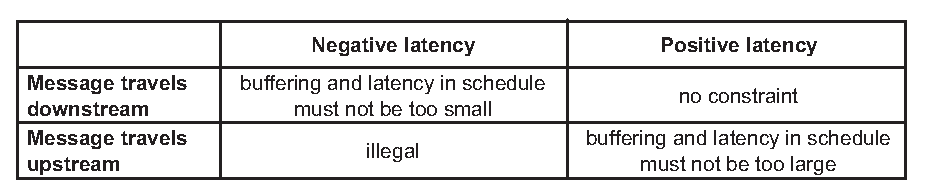
\psfig{file=constraints.eps,width=3in}
\vspace{-4pt}
\caption{\small Scheduling constraints imposed by messages.}
%% {\small
%% \begin{tabular}{|r|c|c|} \hline
%% ~ & {\bf Negative latency} & {\bf Positive latency} \\ \hline
%% {\bf Message travels downstream} & buffering and latency in schedule must not be too small & no constraint \\ \hline
%% {\bf Message travels upstream} & illegal & buffering and latency in schedule must not be too big \\ \hline
%% \end{tabular}}
\label{tab:messcons}
\end{center}
\vspace{-18pt}
\end{figure}

For upstream messages with negative latency, there always exist
iterations of the sender during which any messages sent are
impossible to deliver.  Consider an iteration of the sender that is
the first to depend on data propagating from the $n$th execution of
the receiver.  A negative-latency message would be delivered
immediately after a {\it previous} iteration of the receiver, but
since iteration $n$ has already fired, the message is impossible to
deliver.  Conversely, a downstream message with positive or zero
latency imposes no constraint on the schedule, as the sender has not
yet produced the data that is synchronized with the message.

\paragraph*{Unsatisfiable Constraints}  
Messaging constraints can be unsatisfiable---that is, assuming a
message is sent on every iteration of the sender's work function,
there does not exist a schedule that delivers all of the messages
within the desired latency range.  Such constraints should result in a
compile-time error.  

Figure~\ref{fig:infeasible} illustrates an example of unsatisfiable
constraints.  Though each messaging constraint is feasible in
isolation, the set of constraints together is unsatisfiable.  The
unsatisfiability is caused by conflicting demands on the buffering
between B and C.  The message from B to C constrains this buffer to
contain at least 10 items, while the message from D to A constrains it
to be empty.  We say that these two constraints {\it overlap} because
the paths from sender to receiver intersect a common actor in the
stream graph.
\begin{figure}[t]
\begin{center}
\psfig{figure=infeasible-messaging.eps,height=1.43in}
\vspace{-8pt}
\caption{{\small Example of unsatisfiable message constraints.  Each
node is annotated with its input and output rate.  Messages are shown
by dotted arrows, drawn from sender to receiver with a given latency.
The constraints are satisfiable in isolation, but unsatisfiable in
combination.  \protect\label{fig:infeasible}}}
\end{center}
\vspace{-13pt}
\end{figure}

\paragraph*{Finding a Schedule}
In the presence of overlapping constraints, we leave to future work
the problem of finding a legal execution schedule (if one exists).
Because overlapping constraints can be detected statically, a given
compiler may choose to prohibit overlapping constraints altogether.
%A discussion of the issues involved appears in a
%thesis~\cite{karczma-thesis} by one of the authors.

\begin{figure}[t]
\vspace{-12pt}
\centering
\psfig{figure=fhr-streamit.eps,width=2.841in}
\vspace{-8pt}
\caption{\small Stream graph of frequency hopping radio with teleport messaging.  
A portal delivers point-to-point latency-constrained messages from the
detectors to the RFtoIF stage.
\protect\label{fig:fhr-streamit}}
\vspace{-12pt}
\end{figure}

\begin{figure}[t]
\vspace{-12pt}
\hspace{-0.2in}\psfig{figure=code-freq1.eps,width=3.5in}
\vspace{-24pt}
\caption{\small Frequency hopping radio with teleport messaging.
Arrows depict the path of messages from the sender to the receiver,
via a portal declared in the top-level stream.
\protect\label{fig:freq1}}
\vspace{-12pt}
\end{figure}


For the case of non-overlapping constraints, a simple modification to
pull scheduling will always result in a legal schedule (if one
exists).  First, note that a pull schedule always satisfies
constraints imposed by upstream messages; because upstream (receiving)
actors execute as little as possible per execution of the downstream
(sending) actor, a message can be forwarded to the receiver
immediately after sending.  The receiver can then store the message
and process it at the appropriate iteration.  For downstream messages,
the pull scheduler is modified to always execute one iteration of the
upstream (sending) actor before any execution of the downstream
(receiving) actor that would exceed the latency range.  If the
upstream actor needs more inputs to fire, then they can always be
generated by actors that are further upstream (via a recursive call to
the pull scheduling algorithm).

As described in Section~\ref{sec:evaluation}, our compiler uses a
simple implementation of messaging in which each sender or receiver
executes in its own thread and waits for possible messages at
appropriate iterations.  This approach does not depend on producing a
serial ordering of the actors at compile time.

%\begin{figure}[t]
\begin{center}
\psfig{figure=constrained-example.eps,height=1.5in}
\caption{{\small Example of construction of a constrained schedule. The $\sdepf{R}{S}$ function for filters $R$ and $S$ is given in Table \ref{tab:sdepconst}. The blob between filters $R$ and $S$ illustrates other possible stream elements. $R$ sends a message to $S$ with latency $[1,2]$. Executions of the blob are omitted, it is assumed that at the point $S$ executes, the blob has drained data provided by $R$.}}
\end{center}
\vspace{-12pt}
\label{fig:sdepconst}
\end{figure}

\begin{table*}[t]
{\small
\begin{tabular}{|c|c|} \hline
{\bf $sdepf{R}{S}$} & {\bf Execs of S} \\ \hline
$9n+2$ & $8n+1$ \\ \hline
$9n+3$ & $8n+2$ \\ \hline
$9n+5$ & $8n+3$ \\ \hline
$9n+5$ & $8n+4$ \\ \hline
$9n+6$ & $8n+5$ \\ \hline
$9n+8$ & $8n+6$ \\ \hline
$9n+9$ & $8n+7$ \\ \hline
$9n+9$ & $8n+8$ \\ \hline
\end{tabular}}
\caption{\small $sdepf{R}{S}$ function for example in Figure \ref{fig:sdepconst}. This particular $\sdep$ function was obtained by setting $push_R=2$, $pop_S=3$ and making the blob between $R$ and $S$ into a filter that pops 3 and pushes 4 every iteration of its work function. No initialization due to peeking is necessary in this example.}
\label{tab:sdepconst}
\end{table*}


Explanation of working of the example:

The example in Figure \ref{fig:sdepconst} illustrates scheduling of a single constraint. The constraint is a message sent upstream with latency $[1,2]$. The resulting schedule consists of two parts, an initialization schedule and a steady state schedule. The initialization schedule is necessary to initialize the constraint, to ensure that the steady schedule can be executed repeatedly forever. Notation used here is: $lastReceived$ denotes the execution of S which sent the last message to be received by R; $n_S$ indicates number of executions of $S$ and $n_R$ indicates number of executions of $R$.

Initialization schedule is computed by executing R $SDEP(minLatency)-1$ number of times, and executing S as many times as possible, given data provided by R. This assures that when the steady schedule starts, all executions of filters will contribute to new message sending and receiving, thus allowing the steady state schedule to execute forever. The initialization schedule does not need to send or receive messages here.

The steady state schedule is computed by executing the receiver R as far as possible without going beyond the boundary of being able to receive message sent by S on execution $lastReceived+1$ (indicated by "Oldest msg to receive" in the figure). Now the sender S is executed as many times as possible, given data provided by R. Now S can receive messages sent by S in its executions $[lastReceived+1 ... \min(n_S, $"Newest msg to receive"$)]$.

"Oldest msg to receive" is equal to $iSDEP(n_R)-maxLatency$. "Newest msg to receive" is equal to $m-minLatency$ with $m$ being the greatest integer such that $SDEP(m) \le n_R$.


\section{Case Study}
\label{sec:casestudy}

To illustrate the pros and cons of teleport messaging, we implemented
a spread-spectrum frequency hopping radio frontend~\cite{harada02} as
shown in Figure~\ref{fig:fhr-streamit}.  A frequency hopping radio is
one in which the receiver switches between a set of known frequencies
whenever it detects certain tones from the transmitter.  The frequency
hopping is a good match for control messages because the hopping
interval is dynamic (based on data in the stream); it spans a large
section of the stream graph (there is a Fast Fourier Transform (FFT)
with 15 child actors, not shown, between the demodulator and the hop
detector); and it requires precise message delivery.  The delivery
must be precise both to meet real-time requirements (as the
transmitter will leave the current frequency soon), and to ensure that
the message falls at a logical frame boundary; if the frequency change
is out of sync with the FFT, then the FFT will muddle the spectrum of
the old and new frequency bands.

A StreamIt version of the radio frontend with teleport messaging
appears in Figure~\ref{fig:freq1}.  The FreqHoppingRadio pipeline
creates a portal and adds the RFtoIF actor as a receiver (lines 45 and
48 respectively).  The portal is passed to the CheckFreqHop stage,
where four parallel detectors send messages into the portal if they
detect a hop in the frequency they are monitoring (lines 32-35).  The
messages are sent with a latency of 6 to ensure a timely transition.
To make sense of the latency, note that $\sdepf{RFtoIF}{D}(n) = 512*n$
for each of the detector actors $D$.  This comes about because the FFT
stage consumes and produces 512 items\footnote{\small Though the FFT is
256-way, the real and imaginary parts are interleaved on the tape,
leading to an I/O rate of 512.}; each detector fires once per set of
outputs from the FFT, but RFtoIF fires 512 times to fill the FFT
input.  Because of this $\sdep$ relationship, messages sent from the
detectors to RFtoIF are guaranteed to arrive only at iterations that
are a multiple of 512.  This satisfies the design criterion that a
given FFT stage will not operate on data that were demodulated at two
separate frequencies.

\begin{figure}[t]
\centering
\psfig{figure=fhr-feedback.eps,width=3.13in}
\caption{\small Stream graph of frequency hopping radio with control
messages implemented manually.  A feedback loop connects the detectors
with the RFtoIF stage, and an item is sent on every invocation to
indicate whether or not a message is present.  The latency and
periodicity of message delivery are governed by the data rates and the
number of items on the feedback
path. \protect\label{fig:fhr-manual}}
\end{figure}

Another version of the frequency hopping radio appears in
Figures~\ref{fig:fhr-manual} and~\ref{fig:freq2}.  This version is
functionally equivalent to the first, except that the control messages
are implemented manually by embedding them in the data stream and
in-
%
\begin{figure}[t]
\vspace{-26pt}
\hspace{-0.2in}\psfig{figure=code-freq2.eps,width=3.5in}
\vspace{-20pt}
\caption{\small Frequency hopping radio with manual feedback loop for
event handling.  Lines that differ from Figure~\ref{fig:freq1} are
marked with an asterisk. \protect\label{fig:freq2}}
\vspace{-12pt}
\end{figure}

\clearpage
\noindent
troducing a feedback loop.  Because the number of items transfered
around the loop must be constant from one iteration to the next, a
data item is sent whether or not there is a message as part of the
algorithm.  The RFtoIF filter checks the values from the loop on every
iteration; if the value is non-zero, it is treated as a message (the
new frequency), while a value of zero is ignored (no message).  The
I/O rate of the RFtoIF filter has been scaled up to ensure that the
messaging information is received at intervals of 512 iterations (as
in the version with portals).  To achieve the desired messaging
latency of 6 frames, $6*256 = 1536$ items are enqueued on the feedback
path prior to execution.

%% As described previously, yet another way to approximate the behavior
%% of messaging is with a direct function call from the detector to the
%% RFtoIF stage.  (Though such a call is disallowed in StreamIt, it could
%% be an option in a different programming model.)  While this approach
%% is simple, it does not have any timing guarantees.  Because the sender
%% and receiver are running in parallel, there is no way for the sender
%% to know when in the course of the receiver's execution the message
%% will be received.  This could cause problems both for algorithm
%% development and for the reliability and predictability of software.

\subsection{Discussion}

Teleport messaging offers several benefits compared to a manual
implementation of equivalent functionality.  While embedding messages
in the data stream is equally precise, it involves several tedious
and error-prone changes, not only to the stream graph but also to the
steady-state execution code within the actors.  In particular, the
manual derivation of the loop delay, adjustment of the actor I/O
rates, and implicit interleaving of data items with control messages
has a negative impact on the readability and maintainability of the
code.  Teleport messaging provides the same level of precision, but
with the simplicity of a method call.

Teleport messaging also has advantages from a compiler standpoint.  By
separating the data-intensive code from the control-oriented code, the
common case of steady-state execution is not sacrificed for
the uncommon case of message processing.  There are no ``dummy items''
serving as placeholders in the static-rate channels.  In addition, by
exposing the message latency as part of the language, the compiler can
infer the true dependences between actor firings and reorder the
execution so long as the message constraints are respected.  The
actual message delivery can be implemented in the most efficient way
for a given architecture.

A final benefit of teleport messaging is the clean interface provided
by the portals.  Since a portal can have multiple receivers, it is
straightforward to send a message that is delivered synchronously to
two actors in parallel streams.  For example, consider a vocoder (an
encoder for voice signals) that is separately manipulating the
magnitude and phase components of a signal.  If something triggers an
adjustment to the speech transformation (e.g., the speaker
requests a change of pitch) then the mask needs to be updated at the
same time relative to data in both parallel streams.  A portal that
contains both components seamlessly provides this functionality.
Finally, portals are useful as an external programming interface; an
application can export a portal based on an interface type without
exposing the underlying actor implementation.

One aspect of teleport messaging might be considered unusual: the
granularity of message delivery can be affected by changes in
granularity elsewhere in the stream graph.  This is evident in the
frequency hopping radio, as the I/O rate of 512 on the FFT implies
that the RFToIF stage will receive messages from CheckFreqHop at most
once every 512 iterations.  (If the FFT were coarsened to 1024-way,
the granularity of messages in RFToIF would increase accordingly.)  In
this case the behavior is desirable, as messages should not interrupt
frame boundaries.  It seems that in many cases, the I/O rates are
meaningful aspects of the program and their influence on message
granularity is appropriate.  Nonetheless, this non-local influence
might come as a surprise to programmers.  If the FFT granularity is
scaled up for a different reason (e.g., caching behavior), the effects
on message granularity might be unwanted.

This suggests that it might be worthwhile, in future work, to
investigate additional mechanisms for programmers to specify the
messaging contract independently of the declared I/O rates.  For
example, a parent stream could override the I/O rates of a child for
the sake of a given $\sdep$ calculation.  The scheduler would deliver
messages according to the parent's expectation of $\sdep$, or report
an error if such delivery is incompatible with the actual I/O rates.

\section{Experimental Evaluation}
\label{sec:evaluation}

\begin{table}[t]
\center
\label{tab:benchmarks}
\vspace{-12pt}
{\tiny
\begin{tabular}{|c|c|c|} \hline
{\bf benchmark}&{\bf description}&{\bf \# of actors}\\ \hline \hline
\texttt{bitonic	} &bitonic sort of 64 integers	&	972 \\ \hline
\texttt{fir	      } &finite impulse response program	&	132 \\ \hline
\texttt{fft-fine	} &fine grained FFT implementation	&	267 \\ \hline
\texttt{fft-coarse} &coarse grained FFT implementation	&	26 \\ \hline
\texttt{3gpp	} &3GPP Radio Access Protocol application	&	105 \\ \hline
\texttt{beamformer} &beamformer with 64 sources and 1 detector& 197 \\ \hline
\texttt{matmult	} &matrix multiplication	&	48 \\ \hline
\texttt{fmradio	} &FM Radio with 10 way equalizer	&	49 \\ \hline
\texttt{filterbank} &simple filterbank program	&	53 \\ \hline
\texttt{filterbank2}&alternate implementation of a filterbank &	37 \\ \hline
\texttt{ofdm	 }& Orthogonal Frequency Division Multiplexor~\cite{spectrumware}	&	16 \\ \hline
\end{tabular}
}
\vspace{-12pt}
\caption{Evaluation benchmark suite.}
\end{table}



\begin{figure*}
\begin{minipage}{3.4in}
\psfig{figure=arm2.eps,width=3.4in}
\caption{Performance of various compilation strategies on a StrongARM.\protect\label{fig:arm-perf2}}
\end{minipage}
\hspace{0.1in}
\begin{minipage}{3.4in}
\psfig{figure=arm1.eps,width=3.4in}
\caption{Full fusion versus \texttt{CAF+scaling+buffer} on a StrongARM.\protect\label{fig:arm-perf}}
\end{minipage}
\end{figure*}

\begin{figure*}
\begin{minipage}{3.4in}
\psfig{figure=p3-2.eps,width=3.4in}
\caption{Performance of various compilation strategies on a Pentium~3.\protect\label{fig:p3-perf2}}
\end{minipage}
\hspace{0.1in}
\begin{minipage}{3.4in}
\psfig{figure=p3-1.eps,width=3.4in}
\caption{Full fusion versus \texttt{CAF+scaling+buffer} on a Pentium~3\protect\label{fig:p3-perf}}
\end{minipage}
\end{figure*}

\begin{figure*}
\begin{minipage}{3.4in}
\psfig{figure=i2-2.eps,width=3.4in}
\caption{Performance of various compilation strategies on an Itanium~2.\protect\label{fig:i2-perf2}}
\end{minipage}
\hspace{0.1in}
\begin{minipage}{3.4in}
\psfig{figure=i2-1.eps,width=3.4in}
\caption{Full fusion versus \texttt{CAF+scaling+buffer} on an Itanium~2\protect\label{fig:i2-perf}}
\end{minipage}
\end{figure*}



In this section we evaluate the merits of the proposed cache-aware
optimizations and buffer management strategies. We use three
different architectures: a 137MHz Strong-ARM-1110, a 600~MHz Pentium~3 and 
a 1.3~GHz Itanium~2. All three processors have 16~Kb primary instruction and data caches.


Our benchmark suite (see Table~\ref{tab:benchmarks}) consists of eleven
different StreamIt applications. They are compiled with the StreamIt
compiler which applies the optimizations described in this paper, and
outputs a functionally equivalent C program that is compiled with
\texttt{gcc} (v3.4, -O3) for the StrongARM and for the Pentium~3 and with
\texttt{ecc} (v7.0, -O3) for the Itanium~2. Each benchmark is
then run five times, and the median user time is recorded.


Figures~\ref{fig:arm-perf2}, ~\ref{fig:p3-perf2} and~\ref{fig:i2-perf2} 
illustrate the performance due to the various compilation strategies. 
Figures~\ref{fig:arm-perf}, ~\ref{fig:p3-perf} and~\ref{fig:i2-perf} 
compare full fusion strategy versus a combination of optimizations 
proposed in our paper. The average execution time due to various compilation 
strategies is displayed at the right side of all six figures and all 
execution times are normalized to the execution time of unoptimized 
StreamIt.


The Figures~\ref{fig:arm-perf2}, ~\ref{fig:p3-perf2} and~\ref{fig:i2-perf2} 
have four bars per benchmark. The first bar labeled {\tt scaling}
represents the performance gains compared to the baseline when multiplicity
scaling is applied to the stream graph. The second graph labeled 
{\tt CAF} shows the performance gains compared to the baseline when 
cache-aware fusion is applied to the stream graph. The third graph
labeled {\tt CAF+scaling} shows the performance gains from applying
multiplicity scaling to actors that have been produced using cache-aware
fusion. The last bar labeled \texttt{CAF+scaling+buffer} shows the
execution time when buffer management optimization is combined with
cache-aware fusion and multiplicity scaling.


Only \texttt{fmradio}, \texttt{filterbank}, \texttt{filterbank2}
and \texttt{ofdm} benchmarks have filters that peek, therefore those are the 
only benchmarks that benefit from optimized buffer management when we 
apply all of the optimizations together. 


Scaling improves performance, with a speedup of 148\% for
StrongARM a speedup of 58\% for Pentium~3 and a speedup of 57\% for Itanium~2 over the baseline for our benchmark suite. 
The 90-10 heuristic works quite well and there is only one instance
where scaling results in a performance degradation. The granularity adjusted
\texttt{3gpp} on StrongARM has a 17\% slowdown due to scaling. The is possibly 
due to a buffer for items in flight between the granularity adjusted
actors overwriting the state of an executing actor in the data cache.
Since StrongARM has no L2 cache then such eviction can be quite expensive.

As we coarsen the actors with cache-aware fusion, scaling results 
in less speedup. The speedup of \texttt{CAF+scaling} over \texttt{CAF} is
90\% for StrongARM, 22\% for Pentium~3 and only 20\% for Itanium~2. 
This is because some actors are implicity scaled by fusion to match 
input/output rates of succesive actors within a fused block. 


%% The Itanium~2 has less speedup possibly
%% because of data and instruction prefetch instructions generated by the 
%% \texttt{ecc} compiler.

%% By comparsion, the scaling results on the 
%% Itanium are more uniform, and in fact, scaling does not degrade the
%% performance of any of the benchmarks in suite. 

%% The discrepancy between
%% the Pentium and Itanium results is likely due to the in-order
%% nature of the latter. Unlike the Pentium which can tolerate a cache
%% miss by issuing instructions out-of-order, the Itanium pipeline stalls
%% when an outstanding memory request is not serviced in time for
%% its consuming instruction to execute. The Itanium VLIW architecture
%% therefore places a greater emphasis on the memory hierarchy, and our
%% locality enhancing optimizations help to bridge the gap between
%% processor and memory speeds.

%% whereas it improved the performance of the applications on the Itanium.

%% a few benchmarks on both platforms.
%% A performance degradation as a result of fusion is generally caused by
%% an increase in the buffer management overhead. 


Cache-aware fusion degrades performance only for \texttt{filter}-
\texttt{bank2} on StrongARM by 6\%. When we combine cache-aware fusion 
with multiplicity scaling, the performance consistently improves. 
The speedup of \texttt{CAF+scaling} over baseline is 250\% on StrongARM,
146\% on Pentium~3 and 144\% on Itanium~2.


%% Note that our benchmark suite
%% includes two implementations of \texttt{FFT}. The first is a
%% fine-grained implementation (\texttt{fft-fine}) and the other is a
%% coarse-grained implementation (\texttt{fft-coarse}). The former
%% benefits more from our cache-aware fusion because there is greater
%% versatility in fusing filters to achieve balanced actors. On the other hand
%% a coarse grained implementation restricts the amount of fusion that
%% can be performed and increases the burden for more efficient buffer
%% management. 


Note that the \texttt{ofmd} benchmark does not benefit from fusion or
scaling. This is because  \texttt{ofmd} has few actors that consume 
and produce a total of 16-66Kb data, therefore actors can not be scaled.
Also there is limited oportunity to fuse actors of \texttt{ofmd} 
benchmark, since there are actors that have an instruction size of 9Kb 
and fusing them with other actors would generate actors that exceed the
insturcion cache.


%% In the case of \texttt{fft-coarse}, the scalar-replacement
%% strategy regains nearly 30-70\% of the performance when applied in
%% conjunction with fusion.


The best results overall are measured when all optimizations are
applied in \texttt{CAF+scaling+buffer}. Note that on StrongARM
\texttt{CAF+scaling+buffer} consistenly outperforms full fusion
strategy (see Figure~\ref{fig:arm-perf}), except for a 43\% slowdown 
for \texttt{3gpp}, this is because our compiler predicts that the
fused version of \texttt{3gpp} will not fit into the instruction cache 
due to a conservative code size estimation, however, the optimized code 
of the fused \texttt{3gpp} turns out to be smaller than predicted and 
fits into the 16Kb instruction cache.


On average \texttt{CAF+scaling+buffer} imporves performance over full 
fusion with a 169\% speedup on StrongARM, a 34\% speedup on Pentium~3 
and only a 6\% speedup on Itanium~2. The reason full fusion is better
for several benchmarks on Pentium~3 and Itanium~2 is that 
full fusion allows large reduction of memory accesses by allowing better 
register allocation accross actor boundaries. In cases where full fusion 
outperforms \texttt{CAF+scaling+buffer}, full-fusion results in up to 50\% 
reduction in memory accesses.


If the cache-aware fusion is modified to allow the code size of a 
granularity adjusted actor to be up to one half of the L2 cache on 
Pentium~3 and Itanium~2, then \texttt{CAF+scaling+buffer} results
move closer to or become equal to results of the full fusion in cases where
previously \texttt{CAF+scaling+buffer} was worse than full-fusion.
This modification only reduces performance of \texttt{CAF+scaling+buffer}
for \texttt{ofdm}, where two actors that have a very low communication 
to computation ratio and large instruction size are fused, thus 
limiting the possibility of memory access reduction. 


%% In this case, the granularity-adjusted actors
%% are scaled to maximize cache locality. In addition, the scalar replacement
%% and copy-shift in conjunction with scaling helps to reduce the overhead of 
%% moving data between actors. As a result, the performance gains can be quite
%% dramatic, ranging up to a 5800\% speedup for \texttt{bitonic} on Pentium~3
%% and up to a 6400\% speedup for \texttt{bitonic} on Itanium~2.



\subsection{Buffer Management}

\texttt{CAF+scaling} is our baseline for evaluating optimized buffer 
management strategies. In \texttt{CAF+scaling} the live items are 
copied to the beginning of the buffer after every execution of a filter 
that has $peek>pop$.

\texttt{CAF+scaling+peekscale} strategy replaces filters that have
$peek>pop$ with an equivalent filter that executes the original filter 
multiple times to make sure that $pop$ is at least $4*(peek-pop)$.
This reduces the overhead of copying live items, since we only copy live 
items once after each execution of the scaled actor.

\texttt{CAF+scaling+mod} strategy uses modular buffers for channels where 
downstream filter has $peek>pop$.

\texttt{CAF+scaling+cutpeek} modifies the CAF algorithm so that two 
adjacent filters are never fused if the downstream filter has 
$peek>pop$. After we apply multiplicity scaling to the 
granularity adjusted actors we apply buffer expansion. The 
live items are copied to the start of the buffer once after executing 
the granularity adjusted actor for the number of times that is equal 
to the global multiplicity scaling. This reduces the overhead of 
copying live items.

\texttt{CAF+scaling+cutpeek+mod} also modifies the CAF algorithm so 
that two adjacent filters are never fused if the downstream filter has 
$peek>pop$ and modular buffers are used for channels 
where downstream filter has $peek>pop$.

We found that on average \texttt{CAF+scaling+cutpeek} works best across 
the 3 platforms and this is the buffer optimizatio included in our 
performance numbers. However, \texttt{CAF+scaling+peekscale} is the 
best strategy for fmradio benchmark and our baseline \texttt{CAF+scaling} 
is best for the filterbank benchmark.




\section{Precise Event Handling}
In this section we describe how $\sdep$ information can be
incorporated into the semantics of a language feature that provides
precise delivery of control messages in stream programs.  Our goal is
to improve both programmer productivity and performance.

The Synchronous Dataflow (SDF) domain is well-suited for applications
that have regular, high-bandwidth communication patterns.  However, in
realistic streaming applications there are also irregular,
low-bandwidth control messages that are used to adjust parameters in
various parts of the stream.  For example, a downstream actor might
detect a high signal-to-noise ratio and send a message to the
communications frontend to increase the amplification.  Or, an actor
at the top of the stream graph might detect an invalid checksum for a
packet, and send a message downstream to invalidate the effects of
what has been processed.  Other examples of control messages include:
periodic channel characterization; adaptive beamforming; initiating a
handoff ({\it e.g.,} to a new network protocol); marking the end of a
large data segment; and responding to user inputs, environmental
conditions, or exceptional states.

Generally speaking, control messages are sent at infrequent and
irregular intervals; however, once they are generated there might be
tight constraints on their delivery.  For example, the message
invalidating the effects of a given packet has to be delivered exactly
in sync with the front of the packet itself; otherwise, valid data
will be lost or invalid data will be allowed to pass.

In the rest of this section, we describe language support for control
messages that makes use of $\sdep$ to achieve precise delivery timing.
We first describe the semantics of the language feature, and then we
compare it against other means of implementing messages for a
frequency hopping radio application.

\subsection{Messaging with SDEP}

The messaging system we describe is included as part of the StreamIt
language~\cite{streamitcc}.  In StreamIt, there are two distinct kinds
of communication between filters during steady state execution: 1)
high-bandwidth dataflow over the FIFO channels in the graph, and 2)
low-bandwidth messaging between pairs of filters\footnote{Messaging
is possible whenever there is a downstream path from either filter to
the other.  Filters running in parallel cannot send messages}.  In
order for filter $A$ to send a message to filter $B$, the following
steps need to be taken:
\begin{itemize}

\item $B$ declares a message handler that will be invoked when the
message arrives, for example:
{\small
\begin{verbatim}
handler increaseGain(float amount) {
  this.gain += amount;
}
\end{verbatim}
}
Message handlers are just like normal functions, except that they
cannot access the input/output channels and they have no return value.

\item A parent stream which contains $A$ and $B$ declares a variable
of type {\tt portal<} $T_B$ {\tt >} which can forward messages to
anything of type $T_B$.  The parent adds $B$ to the portal and passes
the portal to $A$ during initialization.

\item To send a message, $A$ invokes the handler method on the portal
from within its steady state work function.  It includes a range of
latencies at which the message should be delivered.  For example:
{\small
\begin{verbatim}
work pop 1 {
  float val = pop();
  if (val < THRESHOLD) {
    portalToB.increaseGain(0.1) [2:3];
  }
}
\end{verbatim}}

\end{itemize}
The most interesting aspect of the messaging system is the semantics
for message latency.  Because there are many legal orderings of actor
executions, there is no notion of ``global time'' in a stream graph.
The only common frame of reference between concurrently executing
actors is the series of data items that is passed between them.  The
$\sdep$ function captures the data dependences in the graph and
provides a natural means of defining a rendezvous point between two
actors.

Intuitively, the message semantics can be thought of in terms of
attaching tags to data items.  If $A$ sends a message to downstream
filter $B$ with a latency $k$, then this could be implemented by
tagging the items that $A$ outputs $k$ iterations later.  These tags
propagate through the stream graph; whenever an actor inputs an item
that is tagged, all of its subsequent outputs are tagged.  Then, the
message handler of $B$ is invoked immediately after the first
invocation of $B$ that inputs a tagged item.  In this sense, the
message has the semantics of traveling ``with the data'' through the
stream graph, even though it does not have to be implemented this way.

The intuition for upstream messages is similar.  Consider that $B$ is
sending a message with latency $k$ to upstream actor $A$ in the stream
graph.  This means that $A$ will receive the message immediately
following the last invocation of its work function which produces an
item affecting the output of $B$'s $k$th firing, counting the current
firing as 0.  As before, we can also think of this in terms of $A$
tagging items and $B$ observing the tags.  In this case, the latency
constraint says that $B$ must input a tagged item before it finishes
$k$ additional executions.  The message is delivered immediately
following the latest firing in $A$ during which tagging could start
without violating this constraint.

The following definition leverages the $\sdep$ formalism to give a
precise meaning to message timing.

\begin{definition}(Message delivery)
Consider that $A$ sends a message to $B$ with latency range
$[k_1:k_2]$ and that the message is sent during the $n$th invocation
of $A$'s work function.  Then the message handler can be invoked in
$B$ immediately after its work function has fired ${\cal M}(A, B, k_1,
k_2, n)$ times, where ${\cal M}$ is constrained as follows.

There are two cases\footnote{In a feedback path, both cases might apply.  In this event, we assume the message is being sent upstream.}:
\begin{enumerate}

\item There is a path in the stream graph from $A$ to $B$.  Then
${\cal M}$ obeys the following constraints:
\[
\begin{array}{l}
\sdepf{A}{B}({\cal M}(A, B, k_1, k_2, n)) \ge n+k_1\\
\sdepf{A}{B}({\cal M}(A, B, k_1, k_2, n)) \le n+k_2
\end{array}
\]

\item There is a path in the stream graph from $B$ to $A$.  Then
${\cal M}$ obeys the following constraints:
\[
\begin{array}{l}
{\cal M}(A, B, k_1, k_2, n) \ge \sdepf{A}{B}(n + k_1)\\
{\cal M}(A, B, k_1, k_2, n) \le \sdepf{A}{B}(n + k_2)
\end{array}
\]
\end{enumerate}
\end{definition}

\begin{table*}[t]
{\small
\begin{tabular}{|r|c|c|} \hline
~ & {\bf Negative latency} & {\bf Positive latency} \\ \hline
{\bf Message travels downstream} & latency in schedule must not be too small & no constraint \\ \hline
{\bf Message travels upstream} & impossible & latency in schedule must not be too big \\ \hline
\end{tabular}}
\caption{\small Effect of message direction and latency on stream graph execution.}
\label{tab:messcons}
\end{table*}

It is instructive to note that there are distinct categories of
message latencies, each of which poses a different constraint on the
execution of the stream graph (see Figure~\ref{tab:messcons}).  A
negative-latency downstream message has the effect of synchronizing
the arrival of the message with some data that was previously output
by the sender ({\it e.g.,} for the checksum example used above).  The
latency requires the downstream actor not to execute too far ahead, or
else it might process the data before the message arrives.  This
translates to a constraint on the minimum latency between the sender
and receiver actors in the schedule of the program.

Similarly, a positive latency upstream message places a constraint on
the maximum latency between the sender and receiver.  Again the
receiver must be throttled so that it doesn't get too far ahead before
the message arrives; however, because the receiver is upstream of the
sender, this constraint represents the need for a tight coupling
between the two filters' executions.

An upstream message with negative latency is impossible to deliver,
because the data dependences imply that the target iteration has
already passed when the message was sent.  Also, a downstream message
with positive latency imposes no constraint, as it is not possible for
the receiver to have executed yet.

\begin{figure}[t]
\begin{center}
\psfig{figure=constrained-example.eps,height=1.5in}
\caption{{\small Example of construction of a constrained schedule. The $\sdepf{R}{S}$ function for filters $R$ and $S$ is given in Table \ref{tab:sdepconst}. The blob between filters $R$ and $S$ illustrates other possible stream elements. $R$ sends a message to $S$ with latency $[1,2]$. Executions of the blob are omitted, it is assumed that at the point $S$ executes, the blob has drained data provided by $R$.}}
\end{center}
\vspace{-12pt}
\label{fig:sdepconst}
\end{figure}

\begin{table*}[t]
{\small
\begin{tabular}{|c|c|} \hline
{\bf $sdepf{R}{S}$} & {\bf Execs of S} \\ \hline
$9n+2$ & $8n+1$ \\ \hline
$9n+3$ & $8n+2$ \\ \hline
$9n+5$ & $8n+3$ \\ \hline
$9n+5$ & $8n+4$ \\ \hline
$9n+6$ & $8n+5$ \\ \hline
$9n+8$ & $8n+6$ \\ \hline
$9n+9$ & $8n+7$ \\ \hline
$9n+9$ & $8n+8$ \\ \hline
\end{tabular}}
\caption{\small $sdepf{R}{S}$ function for example in Figure \ref{fig:sdepconst}. This particular $\sdep$ function was obtained by setting $push_R=2$, $pop_S=3$ and making the blob between $R$ and $S$ into a filter that pops 3 and pushes 4 every iteration of its work function. No initialization due to peeking is necessary in this example.}
\label{tab:sdepconst}
\end{table*}


Explanation of working of the example:

The example in Figure \ref{fig:sdepconst} illustrates scheduling of a single constraint. The constraint is a message sent upstream with latency $[1,2]$. The resulting schedule consists of two parts, an initialization schedule and a steady state schedule. The initialization schedule is necessary to initialize the constraint, to ensure that the steady schedule can be executed repeatedly forever. Notation used here is: $lastReceived$ denotes the execution of S which sent the last message to be received by R; $n_S$ indicates number of executions of $S$ and $n_R$ indicates number of executions of $R$.

Initialization schedule is computed by executing R $SDEP(minLatency)-1$ number of times, and executing S as many times as possible, given data provided by R. This assures that when the steady schedule starts, all executions of filters will contribute to new message sending and receiving, thus allowing the steady state schedule to execute forever. The initialization schedule does not need to send or receive messages here.

The steady state schedule is computed by executing the receiver R as far as possible without going beyond the boundary of being able to receive message sent by S on execution $lastReceived+1$ (indicated by "Oldest msg to receive" in the figure). Now the sender S is executed as many times as possible, given data provided by R. Now S can receive messages sent by S in its executions $[lastReceived+1 ... \min(n_S, $"Newest msg to receive"$)]$.

"Oldest msg to receive" is equal to $iSDEP(n_R)-maxLatency$. "Newest msg to receive" is equal to $m-minLatency$ with $m$ being the greatest integer such that $SDEP(m) \le n_R$.


\subsection{Case Study}

To illustrate the pros and cons of the messaging system, we
implemented a spread-spectrum frequency hopping radio
frontend~\cite{harada02} as appears in Figure~\ref{fig:fhr-streamit}.
A frequency hopping radio is one in which the receiver switches
between a set of known frequencies whenever it hears certain tones
from the transmitter.  The frequency hop is a good match for control
messages because the hopping interval is dynamic (based on on the data
in the stream); it spans a large section of the stream graph (there is
an FFT between the demodulator and the hop detector); and it requires
precise delivery of messages.  The delivery must be precise both to
meet real-time requirements (as the transceiver will leave the current
frequency soon), and to ensure that the message falls at a logical
packet boundary; if the frequency change is out of sync with the FFT
stage, then the FFT will muddle the spectrum of the old and new
frequency bands.

A StreamIt version of the radio frontend with language support for
messaging appears in Figure~\ref{fig:freq1}.  The Freq\_Hopping\_Radio
pipeline creates a portal and adds the RFtoIF actor as a receiver.
The portal is passed to the Check\_Freq\_Hop stage, where four
parallel detectors send messages into the portal if they detect a hop
to the frequency they are monitoring.  The messages are sent with a
small latency (4-6) to ensure a timely transition.  To make sense of
the latency, note that $\sdepf{RFtoIF}{D}(n) = 64*n$ for each of the
detector actors $D$.  This comes about because the FFT stage consumes
and produces 64 items; each detector fires once per set of outputs
from the FFT, but RFtoIF fires 64 times to fill the FFT input.
Because of this $\sdep$ relationship, messages sent from the detectors
to RFtoIF are guaranteed to arrive only at iterations that are a
multiple of 64.  This satisfies the design criterion that a given FFT
stage will not operate on data that was demodulated at two separate
frequencies.

Another version of the frequency hopping radio appears in
Figures~\ref{fig:fhr-streamit} and~\ref{fig:freq2}.  This version is
functionality equivalent to the first, except that the control
messages are implemented manually by embedding them in the data stream
and introducing a feedback loop.  Because the number of items
transfered around the loop must be constant from one iteration to the
next, a data item is sent whether or not there is a message as part of
the algorithm; a special value of 0 represents that there is no
message on the given iteration (in some other programs, no special
value is available, in which case a structure can be passed through
the stream with a boolean flag indicating whether or not a message is
present).  Then, the RFtoIF filter checks the values from the loop on
every iteration and processes them as a message if they are non-zero.
The I/O rate of the RFtoIF filter has been scaled up to ensure that
the messaging information is received at intervals of 64 iterations
(as in the version with portals).  To achieve the desired messaging
latency, a number of items are enqueued on the feedback path prior to
execution.

Yet another way to approximate the behavior of messaging is with a
direct function call from the detector to the RFtoIF stage.  (Though
such a call is disallowed in StreamIt, it could be an option in a
different programming model.)  While this approach is simple, it does
not have any timing guarantees.  There is no way for the sender to
know when in the course of the target's execution the message will be
received.  This could cause problems both for algorithm development
and for reliability / predictability of software.

\subsection{Discussion}

We believe that the StreamIt messaging system offers several benefits
compared to a manual implementation of equivalent functionality.
While embedding messages in the data stream is equally precise, this
involves several tedious and error-prone changes, not only to the
stream graph but also to the steady state execution code within the
actors.  In particular, the manual derivation of the loop delay,
adjustment of the actor I/O rates, and implicit interleaving of data
items with control messages has a negative impact on the readability
and maintainability of the code.  The messaging construct in StreamIt
provides the same level of precision, but with the simplicity of a
method call.

The messaging construct also has advantages from a compiler
standpoint.  By separating the data-intensive code from the
control-oriented code, the common case of the steady state actor
execution is not sacrificed for the uncommon case of message
processing.  There are no ``dummy items'' serving as placeholders in
on the static-rate channels.  In addition, by exposing the message
latency as part of the language, the compiler can infer the true
dependences between filter firings and reorder the execution so long
as the message constraints are respected.  The actual message delivery
can be implemented in the most efficient way for the given
architecture.

A final benefit of the messaging system is the clean interface
provided by the portals.  Since a portal can have multiple receivers,
it is straightforward to send a message that is delivered
synchronously to two actors in parallel streams.  For example,
consider a vocoder that is separately manipulating the magnitude and
phase components of a signal.  If something triggers an adjustment to
the speech transformation ({\it e.g.,} the speaker requests a change
of pitch) then the mask needs to be updated at the same data-relative
time in both parallel streams.  A portal that contains both components
seamlessly provides this functionality.  Finally, portals are useful
as an external programming interface; an application can export a
portal based on an interface type without exposing the underlying
actor implementation.

\clearpage
\begin{figure}[t]
\psfig{figure=fhr-streamit.eps,width=3.5in}
\caption{\small Stream graph of frequency-hopping radio with language
support for messaging.  A messaging portal delivers point-to-point
latency-constrained messages from the detectors to the RFtoIF stage.
\protect\label{fig:fhr-streamit}}
\end{figure}

\begin{figure}[t]
\scriptsize
\begin{verbatim}
float->float filter RFtoIF(int N, float START_FREQ) {
  float[N] weights;
  int size, count;
  
  init { set_frequency(START_FREQ); }
  
  work pop 1 push 1 {
    push(pop() * weights[count++]);
    count = count % size;
  }
  
  handler set_frequency(float freq) {
    count = 0;
    size  = (int) (N * START_FREQ / freq);
    for (int i = 0; i < size; i++)
      weights[i] = sin(i * pi / size);
  }
}

float->float splitjoin Check_Freq_Hop(int N, 
                                      float START_FREQ, 
                                      portal<RFtoIF> port) {
  split roundrobin(N/4-2, 1, 1, N/2, 1, 1, N/4-2);
  for (int i=1; i<=7; i++) {
    if (i==1 || i==4 || i==7) {
      add Identity<float>;
    } else {
      add float->float filter {
        work pop 1 push 1 {
          float val = pop();
          push(val);
          if (val > hop_threshold)
            port.set_frequency(START_FREQ + 
                               i/7*Constants.BANDWIDTH)
        }
      }
    }
  }
  join roundrobin(N/4-2, 1, 1, N/2, 1, 1, N/4-2);
}

void->void pipeline Freq_Hopping_Radio {
  int   N          = 32;
  float START_FREQ = 2402000000;
  portal <RFtoIF> port;

  add Read_From_AtoD(N);
  add RFtoIF(N, START_FREQ) to port;
  add FFT(N);
  add Magnitude();
  add Check_Freq_Hop(N, START_FREQ, port);
  add Output()
}
\end{verbatim}
\vspace{-12pt}
\caption{\small Frequency hopping radio with language support for event handling. \protect\label{fig:freq1}}
\end{figure}

\clearpage
\begin{figure}[t]
\psfig{figure=fhr-feedback.eps,width=3.5in}
\caption{\small Stream graph of frequency-hopping radio with control
messages implemented manually.  A feedback loop connects the detectors
with the RFtoIF stage, and an item is sent on every invocation to
indicate whether or not a message is present.  The latency and
periodicity of message delivery are governed by the data rates and the
number of items on the feedback
path. \protect\label{fig:fhr-manual}}
\end{figure}

\begin{figure}[t]
\scriptsize
\begin{verbatim}
 float->float filter RFtoIF(int N, float START_FREQ) {
   float[N] weights;
   int size, count;
   
   init { set_frequency(START_FREQ); }
   
*  work pop 3*N push 2*N {
*    // manual loop to 2*N.  Factor of N because messages 
*    // for given time slice come in groups of N; factor 
*    // of 2 for data-rate conversion of Magnitude filter
*    for (int i=0; i<2*N; i++) {
*      push(pop() * weights[count++]);
*      count = count % size;
*    }
*    // manually check for messages; 
*    // special value of 0 encodes no message
*    for (int i=0; i<N; i++) {
*      float freqHop = pop();
*      if (freqHop!=0)
*        set_frequency(freqHop);
*    }
*  }
   
   handler set_frequency(float freq) {
     count  = 0;
     size   = (int) (N * START_FREQ / freq);
     for (int i = 0; i < size; i++)
       weights[i] = sin(i * pi / size);
   }
 }

 float->float splitjoin Check_Freq_Hop(int N, 
                                       float START_FREQ) {
   split roundrobin(N/4-2, 1, 1, N/2, 1, 1, N/4-2);
   for (int i=1; i<=7; i++) {
     if (i==1 || i==4 || i==7) {
       add float->float filter {
*        work pop 1 push 2 {
           push(pop());
*          push(0);
         }
       }
     } else {
       add float->float filter {
*        work pop 1 push 2 {
           float val = pop();
           push(val);
*          if (val > hop_threshold) {
*            push(val);
*          } else {
*            push(0);
*          }
         }
       }
     }
   }
*  join roundrobin(2*(N/4-2), 2, 2, 2*(N/2), 2, 2, 2*(N/4-2));
 }

 void->void pipeline Freq_Hopping_Radio {
   int   N             = 32;
   float START_FREQ    = 2402000000;
   
   add Read_From_AtoD(N);
*  add float->float feedbackloop {
*    // adjust joiner rates to match data rates in loop
*    join roundrobin(2*N,N);
*    body pipeline {
*      add RFtoIF(N, START_FREQ);
*      add FFT(N);
*      add Magnitude();
*      add Check_Freq_Hop(N, START_FREQ);
*    }
*    split roundrobin();
*    // number of items on loop path = latency * N
*    for (int i=0; i<6*N; i++)
*      enqueue(0);
*  }
   add Output()
 }
\end{verbatim}
\vspace{-12pt}
\caption{\small Frequency hopping radio with manual feedback loop for
event handling.  Lines that differ from Figure~\ref{fig:freq1} are
marked with an asterisk. \protect\label{fig:freq2}}
\end{figure}
\clearpage

\subsection{Experimental Evaluation of Messaging}

In order  to evaluate  our messaging methodology,  we compile  the two
implementations      of      the      frequency      hopping      radio
(Figures~\ref{}~and~\ref{}) into  a set of  threads. The message-based
implementation  is compiled  into  28 threads,  whereas the  alternate
version---relying on a feedback-loop for notification---results in 32
threads.  Each  thread implements a  specific component of  the stream
graph  (e.g., filter)  and is  allocated to  a specific  machine  in a
networked computing  cluster.  The cluster consists  of sixteen 750Mhz
Pentium~III workstations, each with  a 256~Kb cache.  The machines are
interconnected  using a  fully switched  high speed  network,  and the
threads     are    allowed     to     communicate    via     dedicated
channels. Specifically, every channel  in the stream graph is assigned
a  unique TCP/IP  connections for  the exchange  of data  and messages
between actors.

In order to perform the thread-to-machine allocation, our {\it
clustering} backend, part of the StreamIt
compiler~\cite{streamit-asplos} infrastructure, applies a partitioning
algorithm~\cite{thies-msp} to reduce the overall application
bottleneck while maximizing the throughput of the output filter in the
stream dependence graph. For the purpose of this paper, throughput is
defined as the number of outputs produced per unit of time.

\begin{figure}[t]
\psfig{figure=throughput-graph.eps,width=3.5in}
\caption{\small Throughput as a function of the number of clusters for
the two implementations of the frequency hopping radio.
\protect\label{fig:fhr-throughput}}
\end{figure}

In Figure~\ref{fig:fhr-throughput},  we report the  throughput for the
two applications along the $y$-axis.  Each data point corresponds to a
specific allocation  of the  threads to the  number of  clusters shown
along the $x$-axis.   Note that due to the  limited parallelism in the
two implementations of the  frequency hopper, increasing the number of
clusters beyond five workstations leads to negligible gains with respect
to throughput.   Nonetheless, the use of messaging  achieves a maximal
throughput   that   is    49.8\%   better   than   its   feedback-loop
counterpart. Furthermore, a detailed analysis of the results indicates
a 35\%  reduction in  the total communication  when messaging  is used
instead of a continuous feedback-loop.

\section{Other SDEP Applications}

We believe that there are many interesting applications for $\sdep$ in
programming language design and implementation.  We summarize four
potential applications below.

\subsection{Specifying Latency Constraints}

The latency range included in the messaging construct can be directly
employed as a declarative way to specify latency constraints between
actors.  For instance, our infrastructure can interpret a directive
such as $\mt{maxLatency}(A, B, k)$ to indicate a maximum latency of
$k$ between actors $A$ and $B$.  To implement this directive, the
schedule is constrained as if there were an upstream message with
latency range $[0,k]$.  This kind of data-centric latency constraint
could be important for reactive applications that need to produce an
output before consuming too many items from the input.

\subsection{Debugging}

An immediate application of $\sdep$ is as part of a graphical
debugging environment for stream programs.  For example, if a user is
stepping through the execution of the work function of actor $B$, it
might become apparent that the errant behavior of $B$ is due to
aspects of the input items that originated in actor $A$.  By utilizing
$\sdep$ information, the debugger can provide the iteration of $A$ in
which the items originated, and the user can continue debugging at
that location.

\subsection{Software-Based Speculation}

Software-based speculation is one approach to improving the
performance of irregular scientific applications~\cite{frank-thesis}.
While the graph-level control flow in Synchronous Dataflow is known at
compile time, there could be unpredictable control flow within the
work function of each actor, and a compiler could attempt to improve
performance by speculatively executing a given path.  However, if the
prediction failed, the results of the speculation might have passed
outside the boundaries of the actor and on to other actors in the
graph.  In this case, $\sdep$ provides an exact count of how many
iterations the downstream actors should roll back in order to arrive
at the original state.

\subsection{Program Transformation}

In the realm of scientific computing, a precise notion of dependences
proved essential for developing a robust suite of program analyses and
optimizations.  Representations such as dependence levels~\cite{AK82},
direction vectors~\cite{wolfe82}, and dependence
polyhedra~\cite{Irig88} were important abstractions because they
provided an efficient way to test the validity of program
transformations.  We believe that a similar abstraction of dependences
is needed for the emerging realm of streaming applications, and
$\sdep$ represents our first step towards this goal.

% implementation goes here -- cluster and constrained
%\section{Cluster Backend}

The cluster backend compiles the StreamIt code to a set of threads
that can be executed on a single computer or a networked cluster. In
order to exchange data threads establish TCP/IP connections. A set of
connections is created that represents the flow of data between
filters, splitters and joiners. A separate set of connections is
established between message sender and message receivers in each
portal.

The connections between message sender and receivers are used for both
transmitting the messages and also for sending credits. Credits
represent the number of iterations that a filter is allowed to execute
and this enforces that messages can be executed at given latency.

If a message is sent following data is written to a socket:

{\scriptsize
\begin{verbatim}
int size; // size of message in bytes, including size field
int index; // index of message handler
int iteration_to_execute_at; // target iteration number or
                             // -1 for best effort messages 
int and float parameters;
\end{verbatim}}

Examples:

{\scriptsize
\begin{verbatim}
(16, 0, -1, 1000)
\end{verbatim}}

A best effort message for handler Nr. 0 with one integer parameter set
to 1000.

{\scriptsize
\begin{verbatim}
(16, 0, 8, 1000)
\end{verbatim}}

A message for handler Nr. 0 that has to be executed before its work
function is invoked 8th time. The Message has one integer parameter equal
to 1000.

If a credit is being sent following data is written to a socket:

{\scriptsize
\begin{verbatim}
int -1; 
int credit; 
\end{verbatim}}

Example:


{\scriptsize
\begin{verbatim}
(-1, 8)
\end{verbatim}}

Node can execute only up to first 8 iterations before receiving additional credit.

To calculate the iteration at which to execute the message $\sdep$
function is embedded into the code for the thread sending the
message. Any $\sdep$ function value can be calculated from few
parameters and $\sdep$ values during the first steady state cycle.

Currently in cluster backend each message is scheduled exactly at the 
latest possible
latency and the rest of latency information is discarded. Taking the
latency interval into account would allow creation of a more efficient
schedule for sending credit messages.

If a message is being sent downstream at a negative maximum latency 
or is being sent upstream with a positive maximum latency
then one needs to coordinate the execution of filters by sending
credits to the message receiver threads. Nodes that are receiving 
credits can only execute up to the maximum credit they have received so far.

In the case of a message being sent downstream with negative latency,
$\sdep$ function is used to compute following information during compile 
time:

\begin{enumerate}
\item Number of iterations the upstream message sender can execute before sending any credits,
\item The schedule of sending credits during the first steady state cycle after the initial iterations described in 1.
\end{enumerate}

We use the information about credits to send during the first steady state 
cycle to figure out the number of credits to send during subsequent steady
state cycles. This data is embedded into the message sender thread.

In the case of a message being sent upstream, 
the $\sdep$ function is used to compute following information during compile 
time:

\begin{enumerate}
\item The initial credit that downstream node sends during initialization,
\item The schedule of sending credits during the first steady state cycle.
\end{enumerate}

We use the information about credits to send during the first steady state 
cycle to figure out number of credits to send during subsequent steady
cycles. This data is embedded into the message sender thread.

\section{Related Work}
\label{sec:related}

% BILL

%Signal~\cite{Signal}, 
%Lucid~\cite{Lucid77}, and
%Occam~\cite{Occam}, and Sisal \cite{sisal}.
%Parallel Haskell~\cite{ph}
In addition to StreamIt, there are a number of stream-oriented
languages drawing from domains such as functional, dataflow, CSP and
synchronous programming~\cite{survey97}.  The Brook language is
architecture-independent and focusses on data
parallelism~\cite{brook04}.  Stream kernels are required to be
stateless, though there is special support for reducing streams to a
single value.  Stream\-C/Ker\-nel\-C is lower level than Brook;
kernels written in KernelC are stiched together in StreamC and mapped
to the data-parallel Imagine processor~\cite{imagine03ieee}.  SPUR
adopts a similar decomposition between ``microcode'' stream kernels
and skeleton programs to expose data parallelism~\cite{spur05samos}.
Cg exploits pipeline parallelism and data parallelism, though the
programmer must write algorithms to exactly match the two pipeline
stages of a graphics processor~\cite{cg03}.  Compared to these
languages, StreamIt places more emphasis on exposing task and pipeline
parallelism (all the languages expose data parallelim).
%and on sliding window operations (filters that peek).  
By adopting the synchronous dataflow model of execution~\cite{lee87},
StreamIt focusses on well-structured programs that can be aggressively
optimized.  The implicit infinite loop around programs is also a key
StreamIt characteristic that enables the transformations in this
paper.  Spidle is also a recent stream language that was influenced by
StreamIt~\cite{spidle03}.
%and Lucid Synchrone~\cite{Lucid-Synchrone}.
%Synchronous languages which
%target embedded applications include Esterel~\cite{Esterel},
%Lustre~\cite{Lustre}, and Additional

Liao et al. map Brook to multicore processors by leveraging the affine
partitioning model~\cite{liao06brook}.  While affine partitioning is a
powerful model for parameterized loop-based programs, in StreamIt we
simplify the problem by fully resolving the program structure at
compile time.  This allows us to schedule a single steady state using
flexible, non-affine techniques (e.g., simulated annealing) and to
repeat the found schedule for an indefinite period at runtime.
Gummaraju and Rosenblum map stream programs to a general-purpose
hyperthreaded processor~\cite{gummaraju05micro}.  Such techniques
could be integrated with our spatial partitioning to optimize per-core
performance.  Gu et al. expose data and pipeline parallelism in a
Java-like language and use a compiler analysis to efficiently extract
coarse-grained filter boundaries~\cite{du03sc}.  Ottoni et al. also
extract decoupled threads from sequential code, using hardware-based
software pipelining to distribute the resulting threads across
cores~\cite{ottoni05decoupled}.  By embedding pipeline-parallel
filters in the programming model, we focus on the mapping step.

%%%%%%%%%%%%%%%%%%%%%%%%%%%%%%%%%%%%%%%%%%%%%%%%%%%%%%%%%%%%%%%%%%%%%

Previous work in scheduling computation graphs to parallel targets has
focused on partitioning and scheduling techniques that exploit task
and pipeline parallelism~\cite{SDFSched, SDFSched2,may87communicating,
DAGSched, pipeline-sdf}.  Application of loop-conscious
transformations to coarse-grained dataflow graphs has been
investigated.  Unrolling (or ``unfolding'' in this domain) is employed
for synchronous dataflow (SDF) graphs to reduce the initiation
interval but they do not evaluate mappings to actual
architectures~\cite{unfolding,unfolding2}. Software pipelining
techniques have been applied to SDF graphs onto various embedded and
DSP targets~\cite{bakshi99,chatha-02}, but has required programmer
knowledge of both the application and the architecture. To our
knowledge, none of these systems automatically exploit the combination
of task, data, and pipeline parallelism.  Furthermore, these systems
do not provide a robust end-to-end path for application
parallelization from a high-level, portable programming language.

%% Previous work on instruction-level software pipelining has focused
%% mostly on scheduling machine instructions in a loop via modulo
%% scheduling~\cite{rau81,lam-softpipe}.  The algorithms devised must
%% account for tight resource constraints and complex instruction
%% dependences. Our software-pipelining problem is much less constrained,
%% enabling us to employ a simple greedy heuristic.  

%% Furthermore, a traditional modulo scheduling algorithm is not needed
%% because we have an implicit loop barrier at the end of each
%% steady-state.  ILP compilers for clustered VLIW
%% architectures~\cite{Bulldog,Multiflow,lee98spacetime,qian02} must
%% partition instructions and assign them to clusters as part of the
%% instruction scheduling. Clustering is analogous to our application of
%% filter fusion in our software pipelining algorithm.

\section{Conclusion}
\label{sec:conclusion}

In this paper, we describe the StreamIt compiler for the Raw
architecture.  The stream graph of a StreamIt program exposes the data
communication pattern to the compiler while the lack of global
synchronization frees the compiler to radically reoganize the program
for efficient execution on the underline architecture. The StreamIt
compiler demonstrates the power of this flexibility by totally
reoganizing large programs for better load balance. We were able to
map many of programs on to the Raw processor and obtain good
performance.

We introduce a collection of optimizations, vertical and horizontal
filter fusion, vertical and horizontal filter fission and filter
reordering transformations, that can be used to restructure stream
graphs.  We show that by applying these transformations we can map a
high-level stream program, written to reflect the composition of the
application, onto Raw and achieve good processor utilization and load
balance, leading to a factor of three speedup on two applications.

Unlike all previous streaming languages, the structured streams of
StreamIt makes it possible for us to approach the optimization and
parallelization problems in a very systermatic manner. It enables us
to define multiple optimizations -- targetting different constructs
and requirements -- and to compose them them in a hirearchical manner.

The ability to do global transformations across multiple filters, that
may have originated from very different parts of the application,
makes it possible for the compiler to find optimization opportunities
that may ellude even an experience programmer.  Such capabilities
enables the programmers to write protable streaming applications and
map them efficiently onto any given architecture. This has the
potential of creating a programming standard for emerging
communication exposed architectures.  The StreamIt compiler takes a
fist step towards this goal.



{\small
  \bibliographystyle{abbrv}
  \bibliography{references}
}

%\section{APPENDIX}

%\begin{figure}[t]
\begin{center}
\psfig{figure=constrained-example.eps,height=1.5in}
\caption{{\small Example of construction of a constrained schedule. The $\sdepf{R}{S}$ function for filters $R$ and $S$ is given in Table \ref{tab:sdepconst}. The blob between filters $R$ and $S$ illustrates other possible stream elements. $R$ sends a message to $S$ with latency $[1,2]$. Executions of the blob are omitted, it is assumed that at the point $S$ executes, the blob has drained data provided by $R$.}}
\end{center}
\vspace{-12pt}
\label{fig:sdepconst}
\end{figure}

\begin{table*}[t]
{\small
\begin{tabular}{|c|c|} \hline
{\bf $sdepf{R}{S}$} & {\bf Execs of S} \\ \hline
$9n+2$ & $8n+1$ \\ \hline
$9n+3$ & $8n+2$ \\ \hline
$9n+5$ & $8n+3$ \\ \hline
$9n+5$ & $8n+4$ \\ \hline
$9n+6$ & $8n+5$ \\ \hline
$9n+8$ & $8n+6$ \\ \hline
$9n+9$ & $8n+7$ \\ \hline
$9n+9$ & $8n+8$ \\ \hline
\end{tabular}}
\caption{\small $sdepf{R}{S}$ function for example in Figure \ref{fig:sdepconst}. This particular $\sdep$ function was obtained by setting $push_R=2$, $pop_S=3$ and making the blob between $R$ and $S$ into a filter that pops 3 and pushes 4 every iteration of its work function. No initialization due to peeking is necessary in this example.}
\label{tab:sdepconst}
\end{table*}


Explanation of working of the example:

The example in Figure \ref{fig:sdepconst} illustrates scheduling of a single constraint. The constraint is a message sent upstream with latency $[1,2]$. The resulting schedule consists of two parts, an initialization schedule and a steady state schedule. The initialization schedule is necessary to initialize the constraint, to ensure that the steady schedule can be executed repeatedly forever. Notation used here is: $lastReceived$ denotes the execution of S which sent the last message to be received by R; $n_S$ indicates number of executions of $S$ and $n_R$ indicates number of executions of $R$.

Initialization schedule is computed by executing R $SDEP(minLatency)-1$ number of times, and executing S as many times as possible, given data provided by R. This assures that when the steady schedule starts, all executions of filters will contribute to new message sending and receiving, thus allowing the steady state schedule to execute forever. The initialization schedule does not need to send or receive messages here.

The steady state schedule is computed by executing the receiver R as far as possible without going beyond the boundary of being able to receive message sent by S on execution $lastReceived+1$ (indicated by "Oldest msg to receive" in the figure). Now the sender S is executed as many times as possible, given data provided by R. Now S can receive messages sent by S in its executions $[lastReceived+1 ... \min(n_S, $"Newest msg to receive"$)]$.

"Oldest msg to receive" is equal to $iSDEP(n_R)-maxLatency$. "Newest msg to receive" is equal to $m-minLatency$ with $m$ being the greatest integer such that $SDEP(m) \le n_R$.



%\appendix
\clearpage
%%\section{StreamGraphs}

% This appendix has all of the stream graphs for the 
% benchmark programs used in the paper

\begin{figure*}[t]
  \center
  %{\bf Appendix A: Benchmark Stream Graphs} \\ ~ \\ ~ \\
  \begin{tabular}{ccc}
    \begin{minipage}{3in}
      \center
      \begin{tabular}{cc}
	\begin{minipage}{1.2in}
	  \center
	  \epsfxsize=1.0in
	  \epsfbox{streamgraphs/fir.ps} 
	\end{minipage} &
	\begin{minipage}{1.2in}
	  \center
	  \epsfxsize=1.0in
	  \epsfbox{streamgraphs/sample.ps}
	\end{minipage}\\
      \end{tabular}
    \end{minipage} & ~\hspace{0.5in} & 
    \begin{minipage}{3in}
      \center
      \epsfysize=1.8in
      \epsfbox{streamgraphs/target.ps} 
    \end{minipage}  
    \\
    \begin{tabular}{cc}
      \begin{minipage}{1.2in}
	\center
	{\bf a) FIR} 
      \end{minipage} &
      \begin{minipage}{1.2in}
	\center
	{\bf b) RateConvert} 
      \end{minipage}\\
    \end{tabular} & &
    \begin{minipage}{3in}
      \center
      {\bf c) TargetDetect}
    \end{minipage}
    \\~\\

    \multicolumn{3}{c}{
      \begin{tabular}{cc}
	\begin{minipage}{4in}
	  \center
	  \epsfysize=1.8in
	  \epsfbox{streamgraphs/fm.ps}
	\end{minipage} &
	\begin{minipage}{2in}
	  \center
	  \epsfysize=1.8in
	  \epsfbox{streamgraphs/vocoder.ps}
	\end{minipage} \\
      {\bf d) FM} & {\bf e) Vocoder} \\
      \end{tabular}
    }
    
    \\~\\

    \multicolumn{3}{c}{
      \begin{tabular}{cc}
	\begin{minipage}{5in}
	  \center
	  \epsfxsize=5.0in
	  \epsfbox{streamgraphs/bf.ps}
		  {\bf f) Radar}
	\end{minipage} &
	\begin{minipage}{1in}
	  \center
	  \begin{tabular}{c}
	    \epsfxsize=0.5in
	    \epsfbox{streamgraphs/oversampler.ps} \\
            {\bf g) Oversample} \\
	  \end{tabular}
	\end{minipage} \\
      \end{tabular}
    }
  
    \\~\\

    \begin{minipage}{2.5in}
      \center
      \epsfysize=2.5in
      \epsfbox{streamgraphs/onebit.ps}
    \end{minipage} &  &
    \begin{minipage}{3in}
      \center
      \epsfysize=2.5in
      \epsfbox{streamgraphs/fb.ps}
	
    \end{minipage}
    \\
    {\bf h) OneBit}  & & 
    {\bf i) FilterBank}
    \\
 
    
  \end{tabular}
  \caption{Benchmark Stream Graphs.}
  \label{fig:streamgraphs}
\end{figure*}

\clearpage
%{\bf Appendix C:  Frequency Replacement Scaling} \\ ~ \\ ~ \\



\begin{figure*}[t]
\center
\begin{minipage}{3.4 in}
\center
\epsfxsize=2.2in
\epsfbox{images/frequency-win-theory.eps} \\
{\bf (a): Theoretical}
\end{minipage} 
\begin{minipage}{3.4 in}
\center
\epsfxsize=2.2in
\epsfbox{images/frequency-win-empirical.eps} \\
{\bf (b): Empirical}
\end{minipage}
\caption{Plots showing the theoretical and empirical multiplication reduction factor as a function of the size of the FIR ($M$) and the number of outputs produced per calculation ($N$). The dark regions denote an increase in the required number of multiplications and the light regions a reduction.}
\label{fig:frequency-win}
\end{figure*}

Frequency replacement is an effective optimization because the asymptotic bounds for 
frequency domain computation is lower than the bound for the time domain computation. 
We determined empirically the point at which frequency replacement improves performance.
  
Direct convolution requires $O(MN)$ multiplies. 
The FFT requires $O(N+2(M-1))lg(N+2(M-1))$ multiplications for both the
conversion to and from the frequency domain, and multiplying two $N+2(M-1)$
vectors in the frequency domain requires $O(N+2(M-1))$ multiplications. 
Direct convolution produces $N$ outputs per iteration and the frequency implementation 
produces $N+M-1$ outputs every iteration. 
We define the ``multiplication reduction factor''
to be the number of multiplies required per output using convolution divided by the 
the number of multiplies per output using the frequency transformation.

Figure~\ref{fig:frequency-win}~(a) shows a plot of the theoretical multiplication reduction factor
and Figure~\ref{fig:frequency-win}~(b) shows the same reduction factor measured empirically. 
The roughness in both the theoretical results and the data is due to the fact that
our FFT algorithm requires $N+2(M-1)$ to be a power of two, and the compiler
automatically adjusts $N$ upward to satisfy this requirement. The theoretical 
reduction numbers account for the fact that our implementation requires four 
floating point multiplication operations to perform a complex valued multiply 
in the frequency domain.

Based on the above analysis, our current compiler applies the frequency replacement
transformation on FIR filters that have length $90$ or greater. The target output
rate, $N$, is automatically set to be twice the FIR length.

\end{document}
